\chapter{Results and Discussion}\label{chp:results}

This chapter describes and evaluates the experimental results of this thesis. The prediction accuracy of all models is presented in Section~\ref{sec:predresults}. Section~\ref{sec:featimp} provides an analysis of feature importance. The scheduling simulation outcomes are presented in Section~\ref{sec:schedresults}, and Section~\ref{sec:discussion} provides a discussion of the key findings in the context of the research questions. For reproducibility purposes, the source code and framework that produced these results can be found on GitHub~\cite{celebi_github}.

\needspace{5\baselineskip}
\section{Prediction Model Performance}
\label{sec:predresults}

In order to provide a progressive ablation design for the experiments, six experiments (A-F) were carried out. In experiments A and B, classical tree-based ensemble methods (Random Forest, XGBoost, and LightGBM) were evaluated using both numeric-only and categorical-augmented feature sets. In experiments C to F, three DL architectures (CNN, LSTM, and CNN-LSTM hybrid) were evaluated under static and sequential (sliding window) framing conditions, as well as with and without categorical features. Table~\ref{tab:predresults} reports the performance of the best-performing model(s) from each experiment on the held-out test set. All metrics reported are calculated based upon the original runtime scale.

Figure~\ref{fig:model-comparison} displays a comparison of the performance of each model. The left-hand side illustrates Test MAE (where a lower value represents better results), while the right-hand side represents Test R\textsuperscript{2} (where a higher value represents better results). By far the greatest improvement in results from Experiment A to B was driven by the addition of categorical encoding. Results from Experiment B, based on tree-based models, consistently outperformed those from other methods. DL models were limited to an R\textsuperscript{2} $\approx$ 0. Temporal or sequence-based models from Experiments E and F yielded negative R\textsuperscript{2} values, which indicate their predictions were worse than a simple mean baseline. Therefore, it can be concluded that the ``categorical boost'' was produced by the inclusion of important feature types such as user identity and GPU type. In conclusion, the results shown above clearly demonstrate that using a tree-based approach for ML models is the most effective way to capture relationships within data sets, specifically those related to the Alibaba GPU cluster workload.

\begin{table}[htbp]
\centering
\caption[Test set prediction performance]{Test set prediction performance of the top-performing models across the six experiments. Exp. A/B = tree-based ML; Exp. C/D = static DL; Exp. E/F = temporal DL. Bold indicates the best result per metric.}
\label{tab:predresults}
\resizebox{\textwidth}{!}{%
\begin{tabular}{llrrrrr}
\hline
\textbf{Exp} & \textbf{Model} & \textbf{MAE (s)} & \textbf{MedAE (s)} & \textbf{RMSE (s)} & \textbf{MAPE (\%)} & \textbf{R\textsuperscript{2}} \\ 
\hline
A & Random Forest (Numeric)         & 4{,}316 & 1{,}508 & 13{,}831 & 16.85 & 0.27 \\ 
A & XGBoost (Numeric)               & 4{,}808 & 1{,}894 & 13{,}965 & 19.02 & 0.26 \\ 
A & LightGBM (Numeric)              & 5{,}212 & 2{,}259 & 14{,}315 & 20.66 & 0.22 \\ 
\hline
B & \textbf{XGBoost (One-Hot)}       & \textbf{3{,}389} & \textbf{1{,}129} & \textbf{11{,}375} & \textbf{10.80} & \textbf{0.51} \\ 
B & LightGBM (Native Cat.)          & 4{,}106 & 1{,}510 & 12{,}147 & 14.55 & 0.44 \\ 
B & Random Forest (One-Hot)         & 4{,}187 & 1{,}888 & 12{,}380 & 15.57 & 0.42 \\ 
\hline
C & CNN (Numeric)                   & 6{,}454 & 3{,}166 & 15{,}715 & 18.60 & $-$0.02 \\ 
C & CNN-LSTM Hybrid (Numeric)       & 7{,}020 & 4{,}359 & 15{,}400 & 28.70 & 0.02 \\ 
C & LSTM (Numeric)                  & 8{,}184 & 6{,}442 & 15{,}562 & 42.16 & 0.00 \\ 
\hline
D & LSTM (One-Hot)                  & 5{,}836 & 1{,}576 & 15{,}057 & 6.51 & 0.06 \\ 
D & CNN-LSTM Hybrid (One-Hot)       & 6{,}618 & 3{,}607 & 14{,}702 & 22.30 & 0.11 \\ 
D & CNN (One-Hot)                   & 6{,}866 & 3{,}717 & 15{,}002 & 23.78 & 0.07 \\ 
\hline
E & LSTM (Numeric Seq.)             & 6{,}923 & 4{,}379 & 15{,}627 & 27.64 & $-$0.01 \\ 
E & CNN (Numeric Seq.)              & 8{,}512 & 6{,}624 & 15{,}712 & 45.20 & $-$0.02 \\ 
E & CNN-LSTM (Numeric Seq.)         & 8{,}907 & 7{,}269 & 15{,}723 & 49.07 & $-$0.02 \\ 
\hline
F & CNN (Categorical Seq.)          & 6{,}704 & 3{,}794 & 15{,}285 & 25.23 & 0.04 \\ 
F & CNN-LSTM (Categorical Seq.)     & 10{,}212 & 9{,}693 & 16{,}083 & 61.12 & $-$0.07 \\ 
F & LSTM (Categorical Seq.)         & 13{,}169 & 13{,}582 & 17{,}562 & 85.66 & $-$0.27 \\ 
\hline
\end{tabular}%
}
\end{table}

\begin{figure}[htbp]
\centering
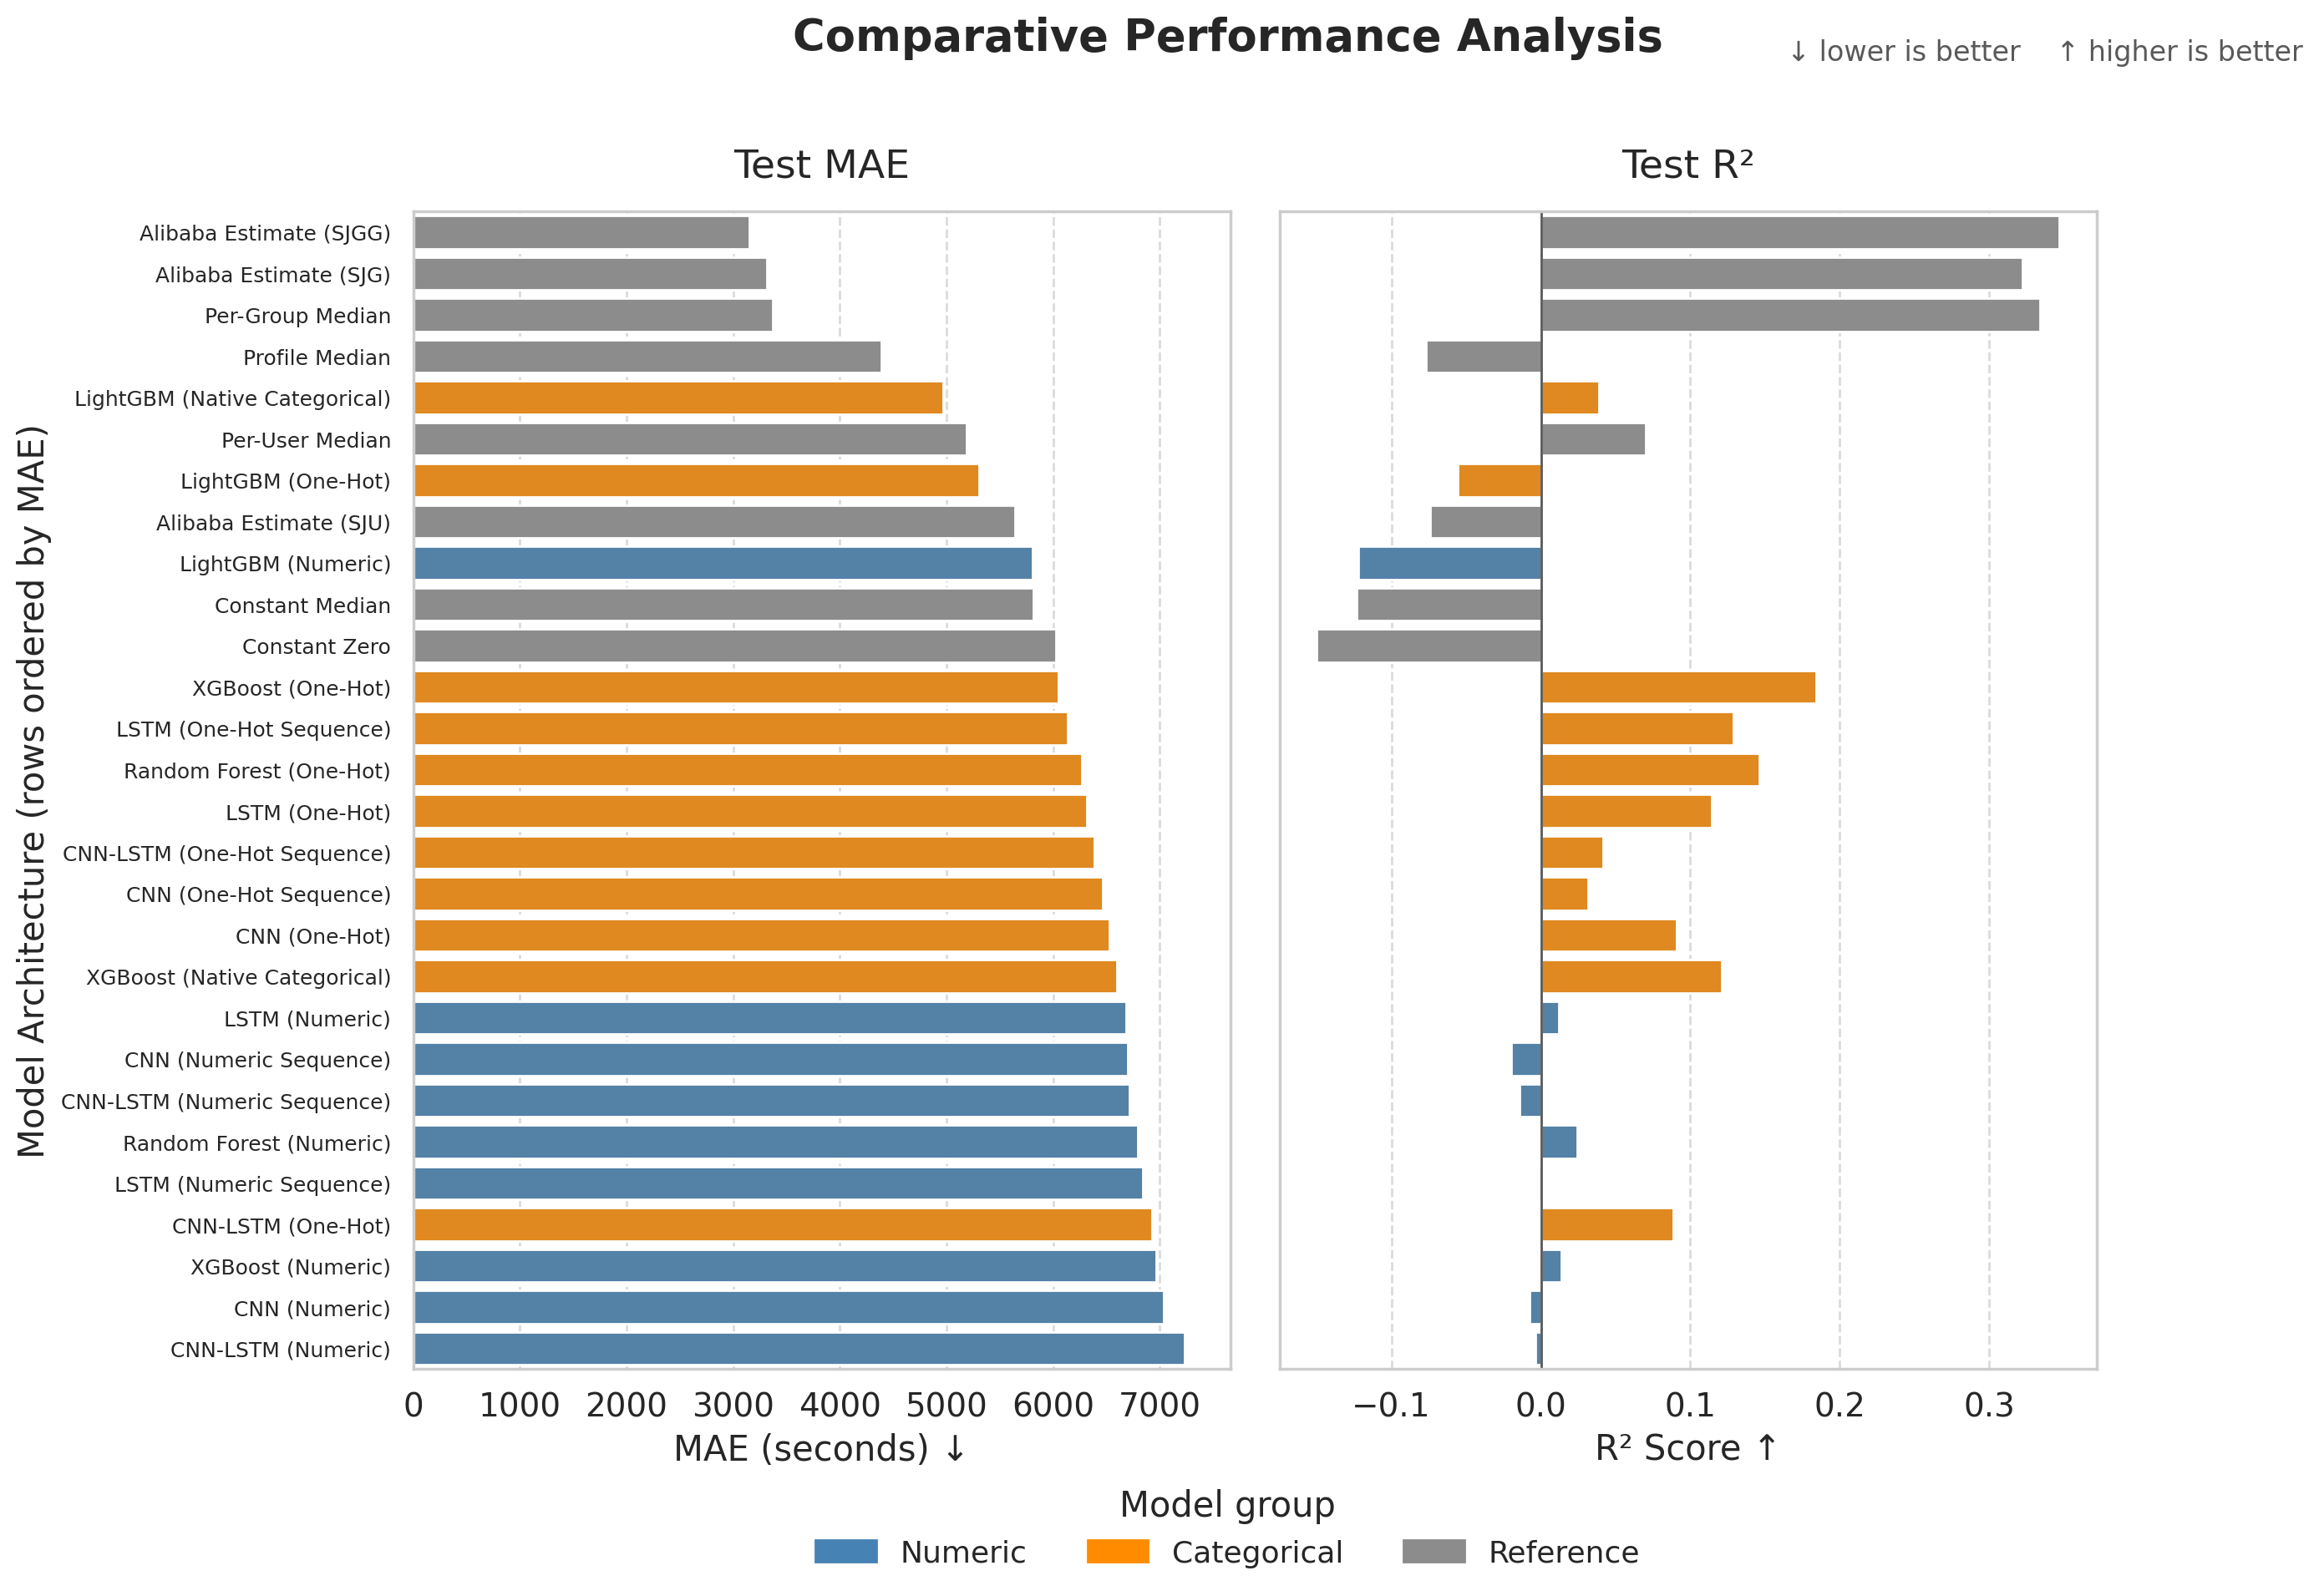
\includegraphics[width=\textwidth]{figures/nb04-fig01-model-comparison.png}
\caption[Comparative performance of all models]{Performance of all models across Experiments A to F.}
\label{fig:model-comparison}
\end{figure}

\subsection{Traditional Machine Learning Model Results}

XGBoost using one-hot encoding (Experiment B) had the highest predictive accuracy out of all of the models tested: MAE of 3{,}389\,s; RMSE of 11{,}375\,s; R\textsuperscript{2} of 0.51. LightGBM (Native Categorical) and Random Forest (One-Hot) followed with R\textsuperscript{2} scores of 0.44 and 0.42, respectively. Adding categorical variables to Experiment B resulted in an improvement in R\textsuperscript{2} of 0.24 compared to the top performing model from Experiment A (Random Forest, R\textsuperscript{2} = 0.27), indicating that both \texttt{gpu\-type} and \texttt{user} identity are significant predictors of performance.

With an R\textsuperscript{2} score of 0.51 for XGBoost, it is clear that the dataset accounts for slightly more than half of the total runtime variance - which is still a relatively high percentage considering the very large variability and long tails in the workload distribution~\cite{weng2022mlaas}.

\subsection{Deep Learning Model Results}

DL architectures (LSTM, 1D-CNN, CNN-LSTM) performed substantially less well than all tree-based models. The results of the DL architectures across experiments C-F are shown in Figure~\ref{fig:dl-comparison}. None of the DL architectures were able to achieve better performance than the best-performing tree-based model (XGBoost with One-Hot encoding, MAE = 3{,}389\,s). In general, time-series-based DL architectures (Experiments E and F) performed significantly less well than their static counterparts. Time series may add noise rather than signal to the training process for this workload as evidenced by the poor performance. The addition of temporal sequencing to these models resulted in no decrease in the absolute error of the predictions made using DL architectures. Instead, the inclusion of temporal sequencing into DL architectures resulted in a significant increase in the MAE, especially for the LSTM architecture, which was structurally unable to effectively process the high-dimensional sparse input matrices. Therefore, while feature representation using one-hot encoding is important to improve DL performance, the static LSTM and the CNN-LSTM hybrid separate only marginally, with the hybrid attaining the higher R\textsuperscript{2}. MAPE is not used to break this tie: on a target spanning five orders of magnitude it is dominated by the shortest jobs and would rank a model with negative R\textsuperscript{2} first. Additionally, complex sequential models have been ineffective in extracting short-term temporal relationships relevant to this workload.

\clearpage
In its best configuration (Experiment D, One-Hot), the LSTM achieved R\textsuperscript{2} = 0.06 and an MAE of 5{,}836\,s. Values of R\textsuperscript{2} ranged from approximately 0.02-0.11 for both the 1D-CNN and CNN-LSTM. However, the application of these sequential models to sliding-window input sequences in Experiments E and F resulted in negative values of R\textsuperscript{2}. A flat prediction of the mean has therefore outperformed these models. A plausible explanation is that sequential models can only add value when the target variable exhibits temporal autocorrelation~\cite{hyndman2021fpp}. Since GPU job runtime lacks temporal autocorrelation in this case, we can conclude that these models are ineffective for this type of problem.

Therefore, the substantial difference in performance between tree-based ensemble models and neural architectures for this type of workload highlights the difficulties in applying deep learning techniques to highly skewed, heterogeneous tabular data. For example, unlike image or text data where deep learning is very good at identifying hierarchically related features, cluster workload trace data is comprised of independent, irregular features with different scales. Neural networks, especially when trained with MAE on heavy-tail distributions, tend to be difficult to optimize due to large amounts of extreme outlier values in the gradient field. Conversely, decision trees are inherently superior due to isolating outliers by recursively dividing the feature space and thus making them much more resilient to extreme execution times associated with ``elephants''. Also, as mentioned earlier, the high dimensionality caused by the use of One-Hot encoding for categorical user and group ID columns results in a very sparse input matrix. Although XGBoost natively handles sparseness during the search for optimal splits in a decision tree due to its sparsity-aware algorithms, feed-forward layers used in the DL architectures suffer from inefficient weight updates and increased sensitivity to overfitting due to their denser structure. Therefore, these structural shortcomings explain why none of the DL architectures were able to outperform XGBoost nor sometimes even perform better than a naive baseline.

\begin{figure}[htbp]
\centering
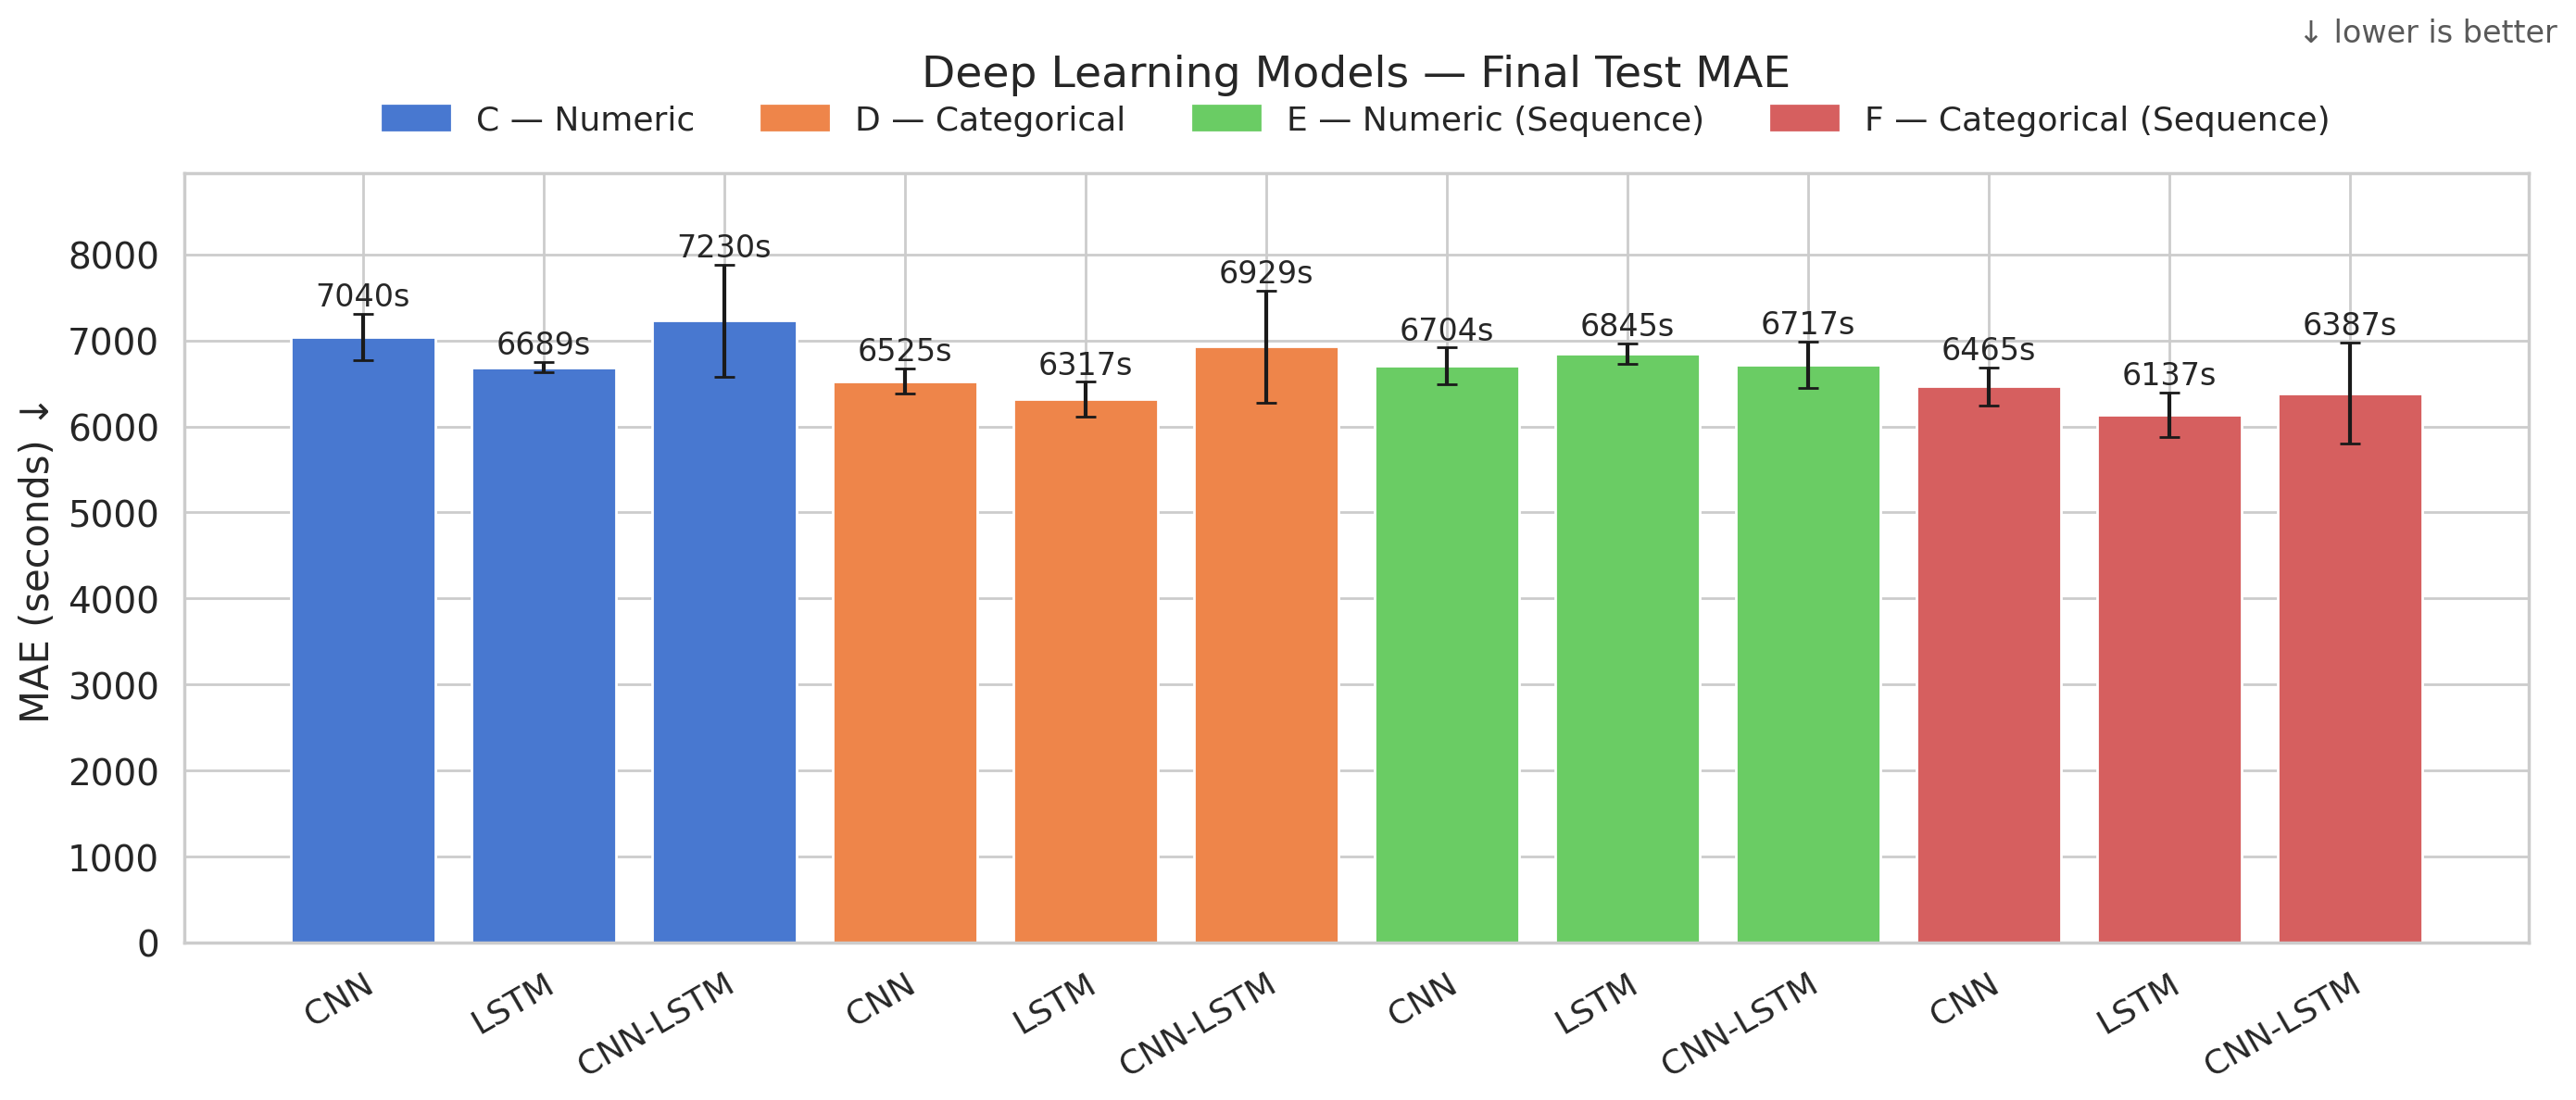
\includegraphics[width=\textwidth]{figures/nb04-fig05-dl-comparison.png}
\caption[Deep learning model performance]{Deep learning model performance across Experiments C, D, E, and F (MAE).}
\label{fig:dl-comparison}
\end{figure}

\needspace{5\baselineskip}
\section{Feature Importance Analysis}
\label{sec:featimp}

Figure~\ref{fig:feature-importance} provides the MDI-based rankings of the three Experiment A tree-based models' numeric features. Each model indicates \texttt{active\-job\-count} as one of the primary indicators of job runtime and validates the inclusion of a real-time cluster usage metric within the feature set. It is also interesting to see how each model assigns relative weightings to the various resource request parameters (e.g., \texttt{gpu\-demand}) to predict job runtimes: Random Forest's emphasis on arrival times, XGBoost's focus on resource requests, and LightGBM's reliance on global metrics regarding system-wide load. All three findings confirm that resource requests and system-wide utilization at the point of job submission provide significant predictive power for accurately modeling job execution time. Additionally, resource-request-based features (i.e., number of GPUs, number of CPUs) have high rankings due to the generally expected inverse relationship between the size of a job and its length. Secondary signals provided by temporal features (e.g., hour of day) assist in distinguishing diurnal patterns in the workloads; \texttt{day\_of\_week} is a trace-relative day counter rather than a calendar weekday (Chapter~\ref{chp:dataset}) and its contribution is better read as a coarse trace-position signal than a weekly-cycle one.

\begin{figure}[H]
\centering
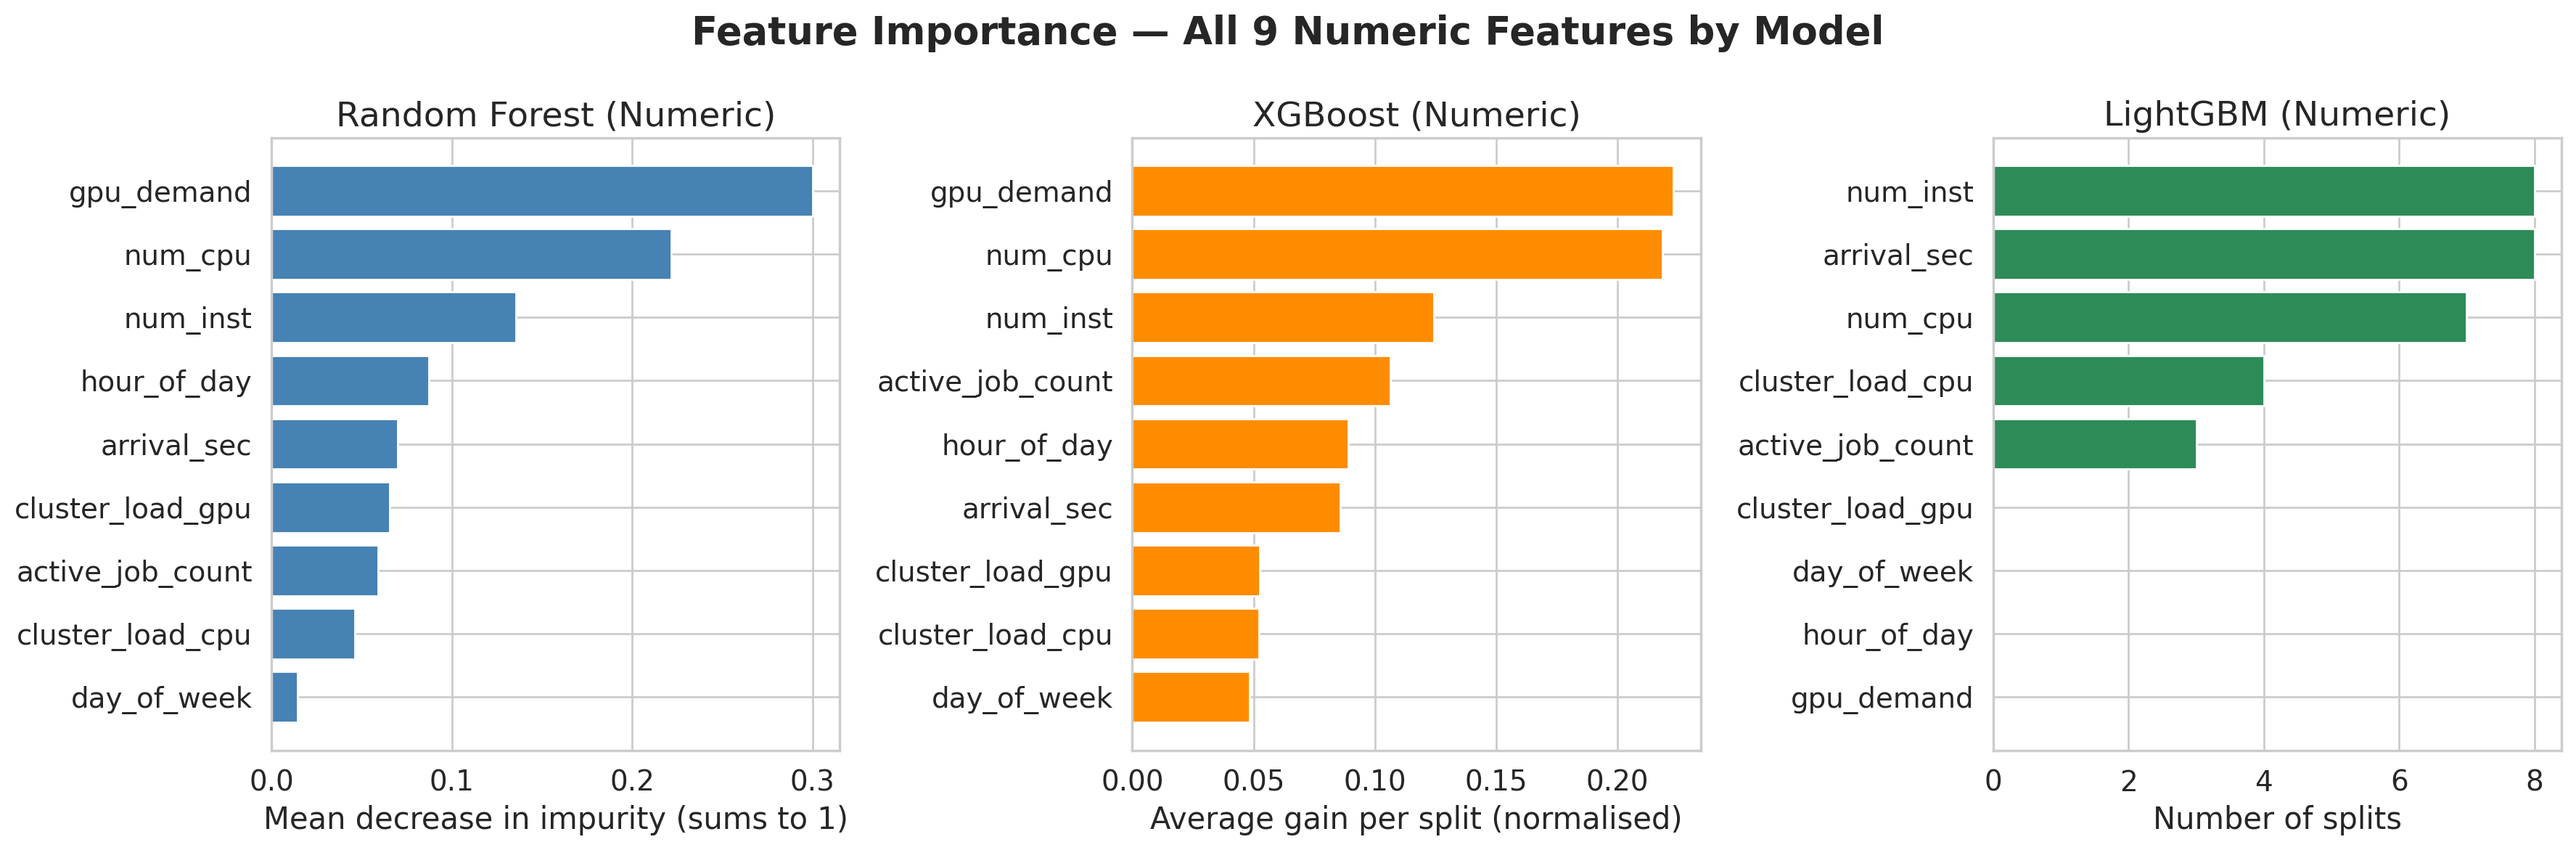
\includegraphics[width=\textwidth]{figures/nb04-fig02-feature-importance.png}
\caption[Feature importance for tree-based models]{Feature importances (MDI-based, all nine numeric features) for Random Forest, XGBoost, and LightGBM trained exclusively on numeric features (Experiment A).}
\label{fig:feature-importance}
\end{figure}

\clearpage
Figure~\ref{fig:pred-vs-actual} depicts predicted versus actual job runtime for the three Experiment A models, with the dashed diagonal line marking a ``perfect'' prediction. An earlier draft of this section reported that most points cluster around that diagonal for short-to-medium jobs, with deviation appearing only in the long tail. That reading does not hold: the sample previously plotted was not random but the chronologically first 3,000 test rows (roughly the first fifth of the test window, a single time slice rather than a representative cross-section), and even within that non-representative sample the three models' predictions sit in a comparatively flat band rather than tracking the diagonal -- consistent with the modest $R^2$ values (0.22-0.27) reported in Table~\ref{tab:predresults} for this experiment, not with a close fit for the bulk of jobs. The figure now plots a genuinely random sample of the test set on log-log axes (chosen because job runtime is heavy-tailed; see Chapter~\ref{chp:dataset}), which is a fairer basis for judging where predictions do and do not track the diagonal; this discussion is being revised to match once the pipeline is re-run under the corrected feature set and tuning objective (Kademe 1).


\begin{figure}[htbp]
\centering
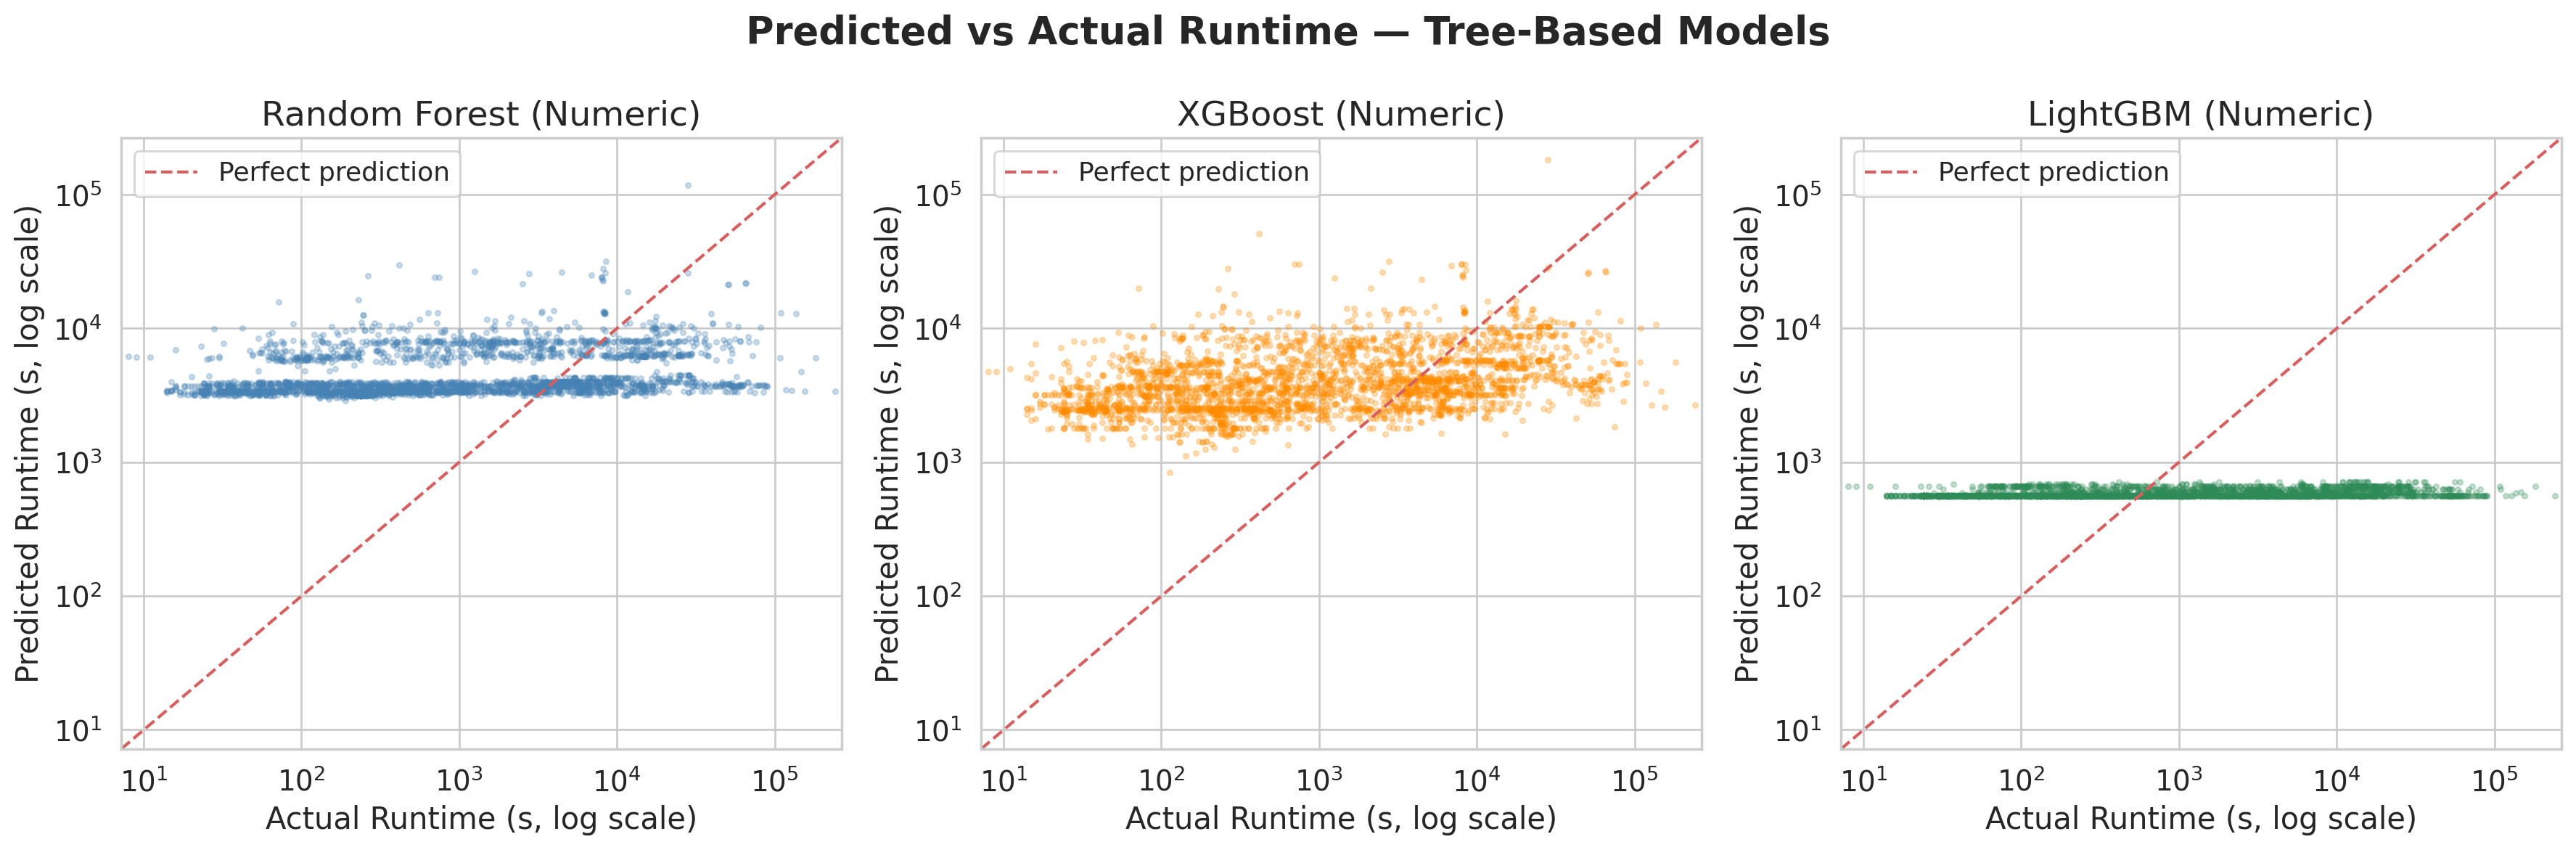
\includegraphics[width=\textwidth]{figures/nb04-fig03-pred-vs-actual.png}
\caption[Predicted vs actual job runtimes]{Predicted versus actual values of job runtimes for Random Forest, XGBoost, and LightGBM, on a random sample of 3,000 test-set jobs (fixed seed) shown on log-log axes to make the heavy-tailed runtime distribution legible. Earlier printings of this figure used the chronologically first 3,000 test rows rather than a random sample.}
\label{fig:pred-vs-actual}
\end{figure}

\clearpage
Figure~\ref{fig:residuals} shows the residual distributions (predicted $-$ actual) for the three Experiment~A tree-based models, demonstrating that none of these models shows a significant positive or negative bias; the residual distribution is generally centered on zero indicating no consistent direction in prediction error. The long tails of the residual distribution indicate that all three models have consistently underestimated the longer running jobs (predicted $-$ actual $< 0$) which is expected due to the fact that we are attempting to predict a variable with a heavy-tail using a relatively small number of features. Figure~\ref{fig:pred-vs-actual} also demonstrates this through the large number of jobs with heavy-tails present in its upper right hand portion. The distributions of both XGBoost and LightGBM residuals are tight and peaked demonstrating their ability to make predictions based on the input data for almost every job with great stability and consistency while the extended tails reflect the inherent variability in the runtime of GPUs and the ongoing challenges associated with estimating extreme values of execution time.

\begin{figure}[htbp]
\centering
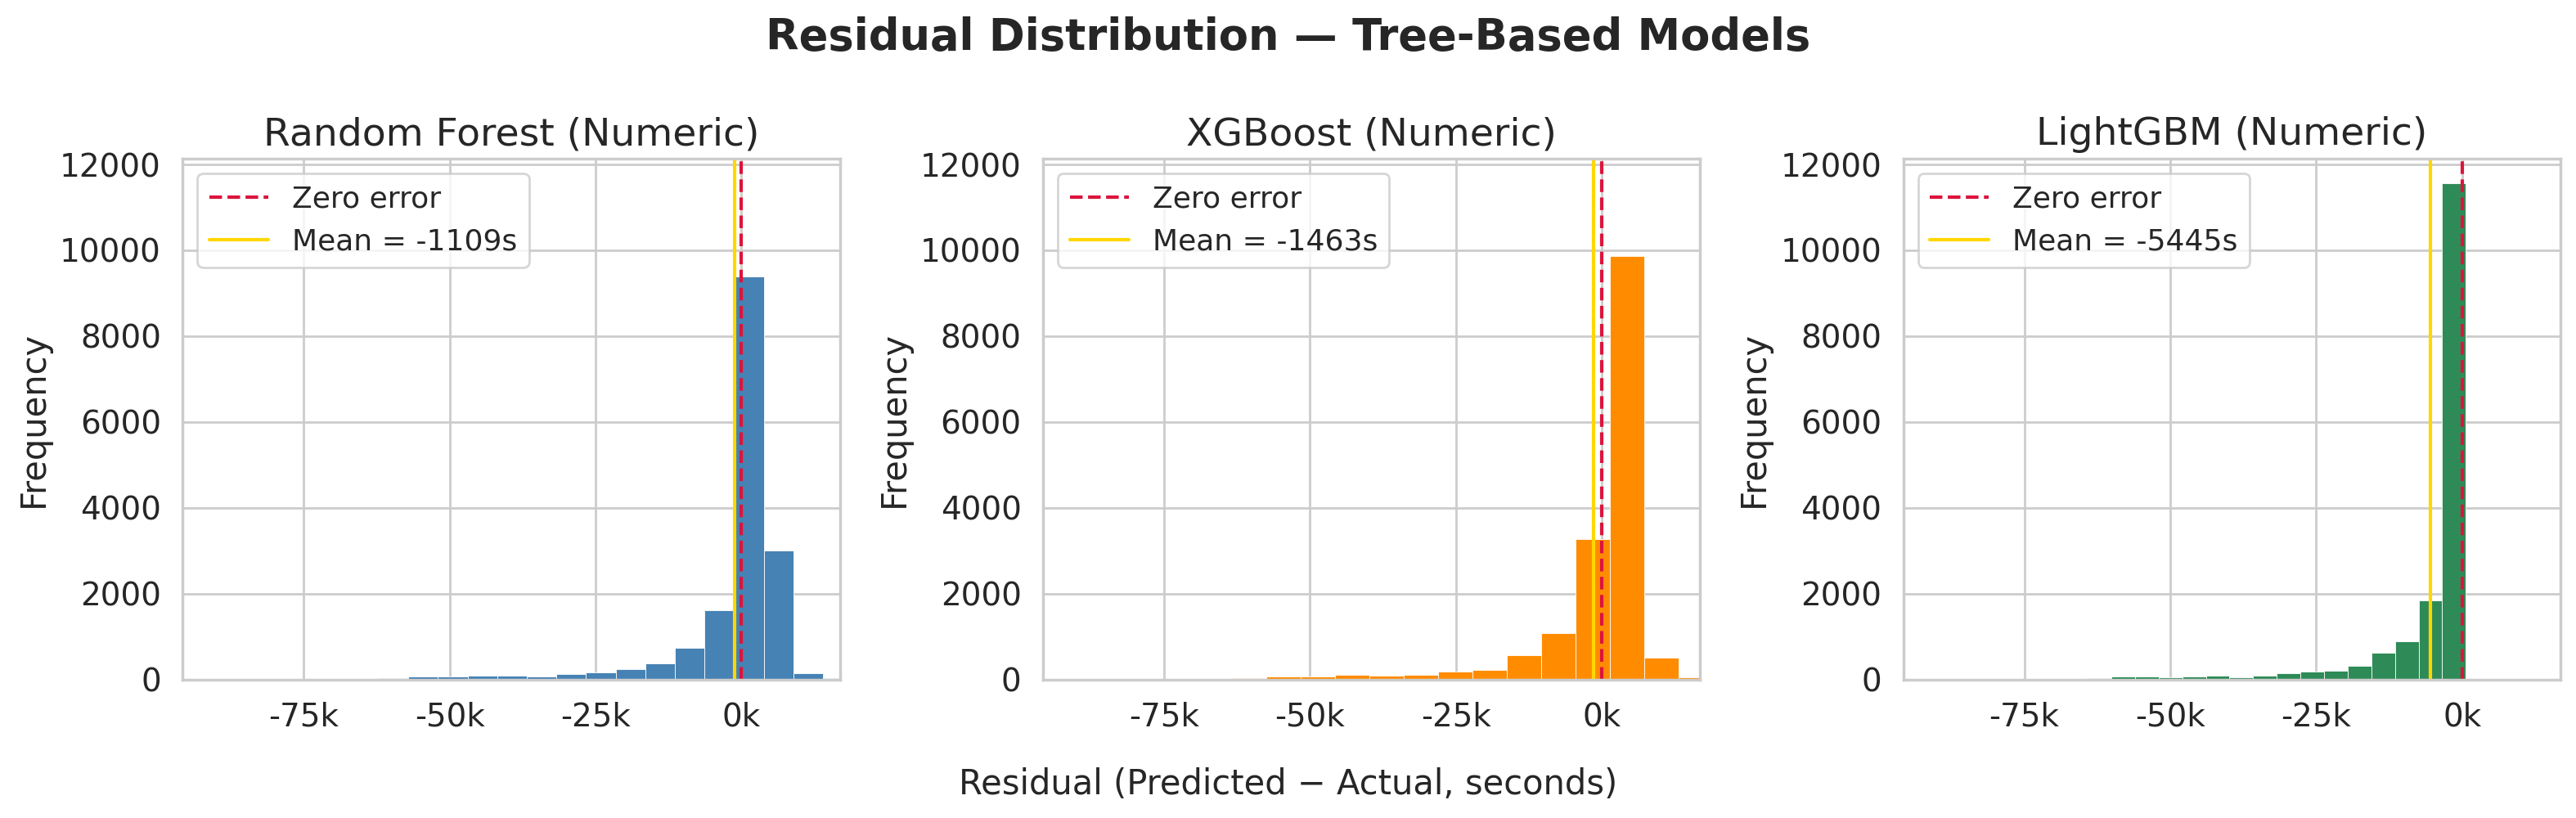
\includegraphics[width=\textwidth]{figures/nb04-fig04-residuals.png}
\caption[Residual distributions]{Residual plots (predicted value minus actual value) for Random Forest, XGBoost, and LightGBM. Each model has residual values centered about zero. XGBoost and LightGBM exhibit narrower residual intervals.}
\label{fig:residuals}
\end{figure}

\needspace{5\baselineskip}
\section{Scheduling Simulation Results}
\label{sec:schedresults}

Table~\ref{tab:schedresults} shows the mean job waiting time and JCT improvement compared to FIFO scheduling for all scheduler-predictor combinations tested with a DES. To evaluate the scalability and robustness of the predictive models under extreme conditions, the DES runs were conducted at an extremely heavy burst load factor (Load Factor = 0.1) on a large-scale (256-GPU), heterogeneous system. In this ``Flash Crowd'' type of traffic pattern, there will be a significant queue bottleneck and the scheduler's ability to manage queues is severely tested. (Models labeled ``One-Hot'' in Table~\ref{tab:predresults} appear as ``Categorical'' below; LGBM (Native Cat.) = SJF-LGBM (Categorical).)

\begin{table}[htbp]
\centering
\small
\caption[Mean job waiting time and JCT improvement]{Mean job waiting time and JCT improvement relative to FIFO of each scheduling policy in both 32-GPU and 256-GPU environments. Results are sorted by mean job waiting time improvement in descending order.}
\label{tab:schedresults}
\resizebox{\textwidth}{!}{%
\begin{tabular}{lrrrr}
\hline
\textbf{Policy / Model} & \textbf{Mean Wait (s)} & \textbf{Mean JCT (s)} & \textbf{JCT Improv. (\%)} & \textbf{Significant?} \\ 
\hline
\multicolumn{5}{c}{\textbf{Small Cluster (32-GPU) Results}} \\
\hline
SJF-Oracle & 86{,}034 & 92{,}064 & 81.59 & --- \\
SJF-XGBoost (Categorical) & 212{,}721 & 218{,}751 & 56.25 & \checkmark \\
SJF-LSTM (Categorical) & 217{,}898 & 223{,}928 & 55.21 & \checkmark \\
SJF-RF (Categorical) & 218{,}787 & 224{,}817 & 55.03 & \checkmark \\
SJF-LGBM (Categorical) & 225{,}571 & 231{,}601 & 53.68 & \checkmark \\
SJF-CNN-LSTM (Categorical) & 226{,}706 & 232{,}736 & 53.45 & \checkmark \\
SJF-CNN (Categorical) & 247{,}446 & 253{,}476 & 49.30 & \checkmark \\
SJF-LGBM (Numeric) & 271{,}686 & 277{,}715 & 44.45 & \checkmark \\
SJF-CNN-LSTM (Numeric) & 286{,}928 & 292{,}958 & 41.40 & \checkmark \\
SJF-CNN-LSTM (Categorical Sequence) & 292{,}565 & 298{,}595 & 40.28 & \checkmark \\
SJF-XGBoost (Numeric) & 316{,}472 & 322{,}501 & 35.49 & \checkmark \\
SJF-LSTM (Numeric) & 321{,}571 & 327{,}601 & 34.47 & \checkmark \\
SJF-CNN (Numeric) & 331{,}494 & 337{,}523 & 32.49 & \checkmark \\
SRF (Heuristic) & 382{,}433 & 388{,}463 & 22.30 & \checkmark \\
SJF-CNN (Categorical Sequence) & 386{,}035 & 392{,}065 & 21.58 & \checkmark \\
SJF-CNN-LSTM (Numeric Sequence) & 394{,}537 & 400{,}567 & 19.88 & \checkmark \\
SJF-LSTM (Categorical Sequence) & 404{,}583 & 410{,}613 & 17.87 & \checkmark \\
SJF-RF (Numeric) & 457{,}949 & 463{,}979 & 7.20 & \checkmark \\
FIFO & 493{,}921 & 499{,}951 & 0.00 & --- \\
SJF-CNN (Numeric Sequence) & 500{,}981 & 507{,}011 & -1.41 & (fail) \\
SJF-LSTM (Numeric Sequence) & 721{,}475 & 727{,}505 & -45.52 & (fail) \\
\hline\hline
\multicolumn{5}{c}{\textbf{Large Cluster (256-GPU) Results}} \\
\hline
SJF-Oracle & 8{,}476 & 14{,}506 & 71.21 & --- \\
SJF-LSTM (Categorical) & 15{,}507 & 21{,}537 & 57.25 & \checkmark \\
SJF-CNN-LSTM (Categorical) & 16{,}402 & 22{,}431 & 55.48 & \checkmark \\
SJF-RF (Categorical) & 17{,}104 & 23{,}133 & 54.09 & \checkmark \\
SJF-XGBoost (Categorical) & 17{,}189 & 23{,}219 & 53.92 & \checkmark \\
SJF-LGBM (Categorical) & 17{,}694 & 23{,}724 & 52.92 & \checkmark \\
SJF-CNN (Categorical) & 17{,}853 & 23{,}883 & 52.60 & \checkmark \\
SJF-LGBM (Numeric) & 20{,}147 & 26{,}177 & 48.05 & \checkmark \\
SJF-CNN-LSTM (Numeric) & 20{,}406 & 26{,}436 & 47.53 & \checkmark \\
SJF-LSTM (Numeric) & 21{,}256 & 27{,}286 & 45.85 & \checkmark \\
SJF-CNN-LSTM (Categorical Sequence) & 24{,}435 & 30{,}465 & 39.54 & \checkmark \\
SJF-CNN (Numeric) & 24{,}469 & 30{,}498 & 39.47 & \checkmark \\
SJF-XGBoost (Numeric) & 24{,}512 & 30{,}542 & 39.38 & \checkmark \\
SJF-CNN-LSTM (Numeric Sequence) & 28{,}948 & 34{,}978 & 30.58 & \checkmark \\
SRF (Heuristic) & 29{,}424 & 35{,}454 & 29.64 & \checkmark \\
SJF-LSTM (Categorical Sequence) & 30{,}189 & 36{,}219 & 28.12 & \checkmark \\
SJF-RF (Numeric) & 38{,}233 & 44{,}262 & 12.15 & \checkmark \\
SJF-CNN (Categorical Sequence) & 39{,}395 & 45{,}425 & 9.85 & \checkmark \\
FIFO & 44{,}356 & 50{,}386 & 0.00 & --- \\
SJF-CNN (Numeric Sequence) & 46{,}425 & 52{,}455 & -4.11 & (fail) \\
SJF-LSTM (Numeric Sequence) & 67{,}236 & 73{,}266 & -45.41 & (fail) \\
\hline
\end{tabular}%
}
\end{table}

\clearpage
Figure~\ref{fig:scheduler-jct} shows the average JCT for all studied policies, at both the small 32-GPU cluster and the large 256-GPU cluster.

An earlier draft of this section reported that tree-based point predictors (LightGBM, XGBoost) delivered the largest scheduling gain at the 32-GPU scale, with the categorical LSTM overtaking them only at the 256-GPU scale. On re-verification against the current checkpoints, this is not what the simulation shows: the categorical LSTM policy achieves the largest JCT improvement over FIFO at \emph{both} cluster sizes, and the ranking of all evaluated policies by JCT improvement is nearly identical between the two scales (Spearman rank correlation above 0.98).\footnote{Exact JCT-improvement and Oracle-capture percentages for every policy at both scales are being refreshed following a code-level correction to the hyperparameter-tuning loss function and the addition of non-learned reference baselines (Per-User Median, Profile Median); see the Limitations section. The corrected LightGBM/XGBoost models are still expected to rank among the strongest categorical policies at both scales -- what does not hold is the claim that they specifically \emph{overtake} the categorical LSTM at the smaller scale.} Tree-based point predictors remain competitive contributors to queue ordering at both scales; what the evidence no longer supports is a scale-triggered reversal in which accuracy-driven ranking wins at 32 GPUs and representation-driven ranking wins only at 256 GPUs.

As previously stated, however, purely numerical sequential DL models fail to achieve the performance of FIFO in a 256-GPU environment. Therefore, they fall victim to the ``sequence trap''. In addition to the ``sequence trap'', temporal features from the sliding window that are uncorrelated with the target variable also cause a disruption to queue rankings. Therefore, simply having a scheduling policy does not guarantee success; proper structuring of one's prediction model is necessary for a successful scheduling policy.

\begin{figure}[htbp]
\centering
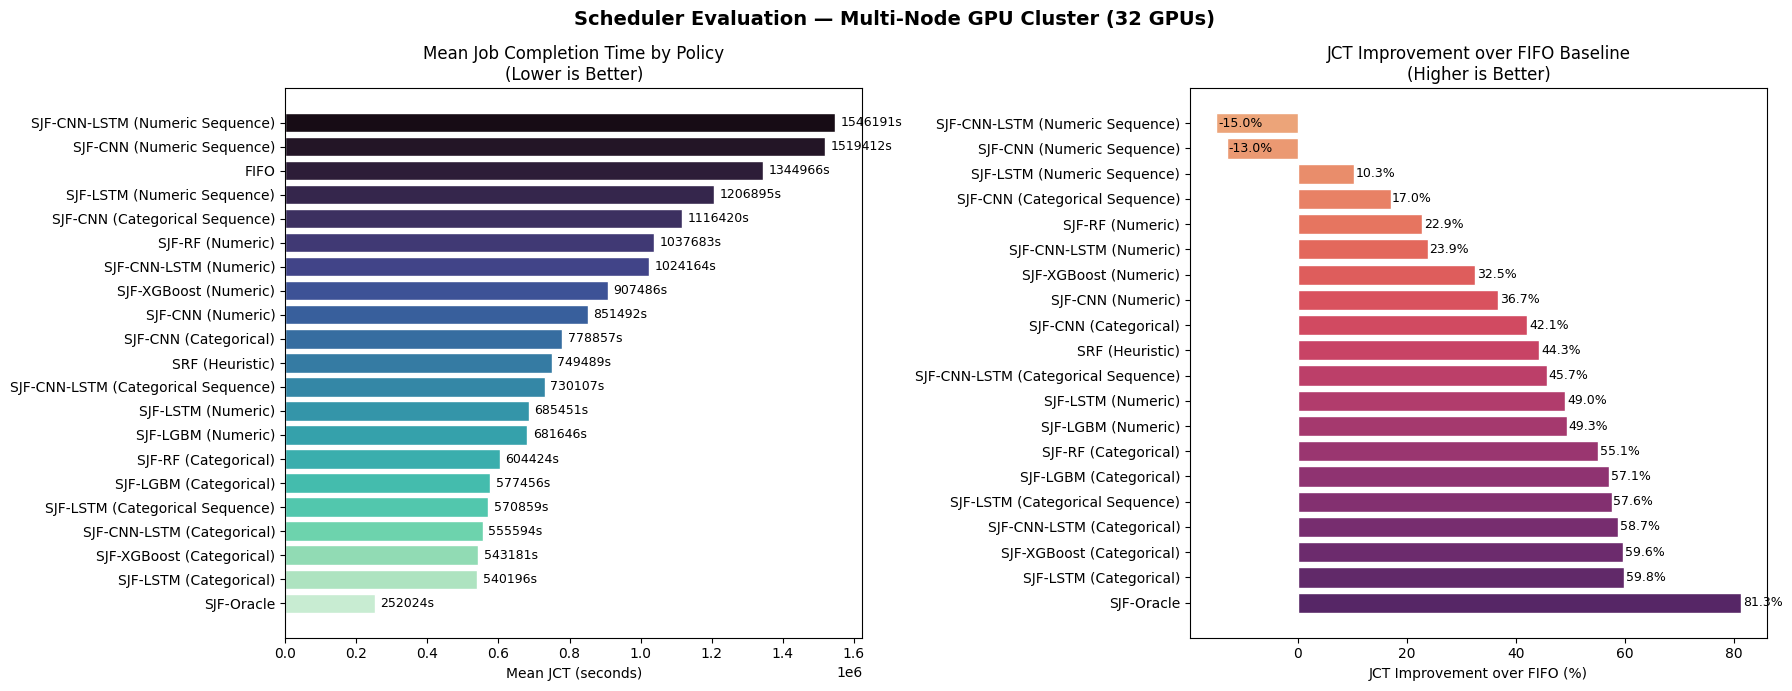
\includegraphics[width=0.48\textwidth]{figures/nb05-fig01-scheduler-jct_32gpu.png}
\hfill
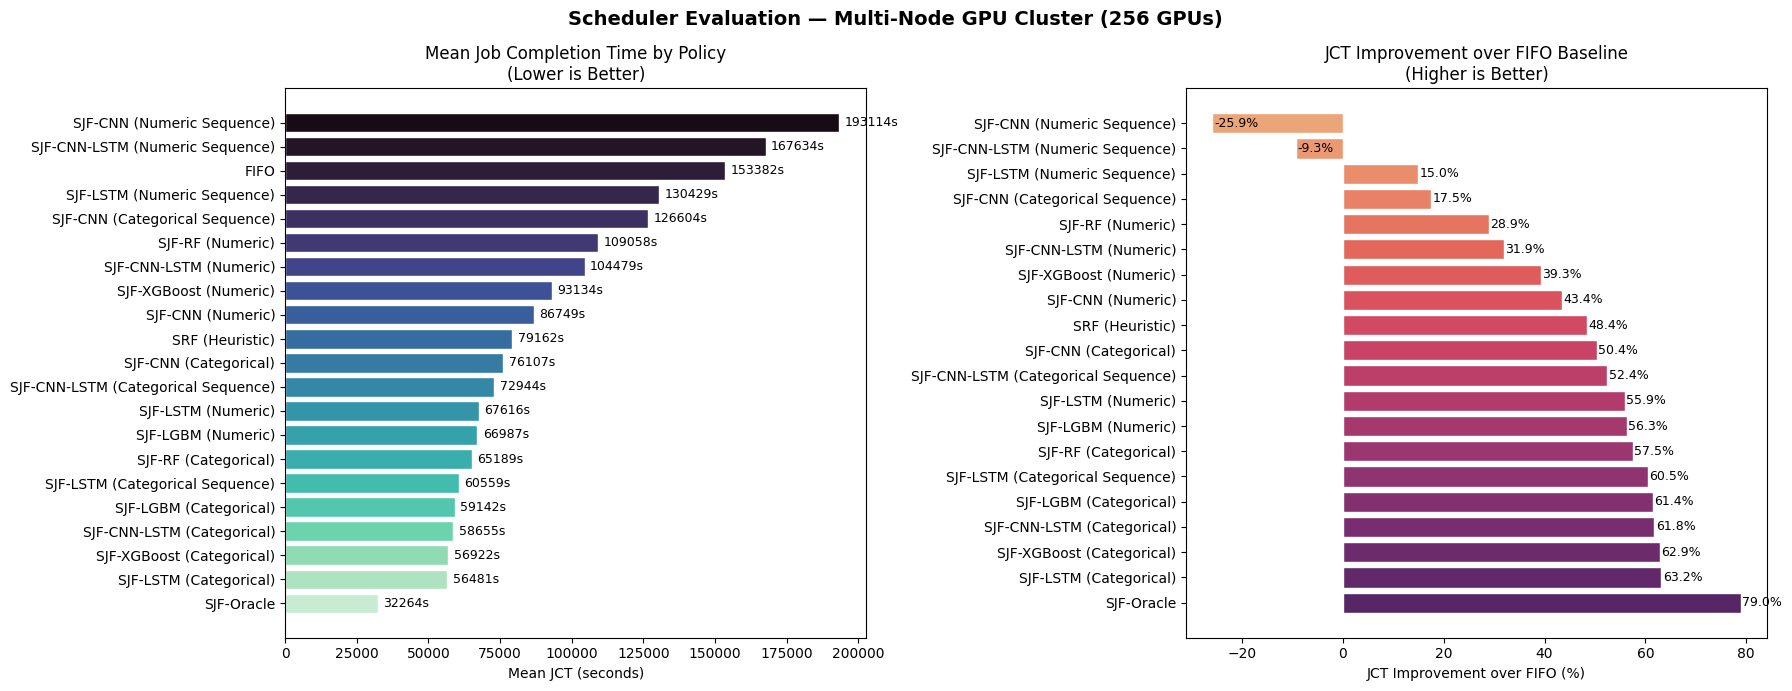
\includegraphics[width=0.48\textwidth]{figures/nb05-fig01-scheduler-jct_256gpu.png}
\caption[Comparative mean JCT]{Comparative average JCT for all policies. The categorical LSTM policy achieves the largest JCT improvement over FIFO at both the small 32-GPU cluster (left) and the large 256-GPU cluster (right); tree-based categorical models are close competitors at both scales.}
\label{fig:scheduler-jct}
\end{figure}

\clearpage
Figure~\ref{fig:improvement-heatmap} provides a visual comparison of how three different scheduling metrics improve compared to each other in terms of scheduling policy improvements when comparing the policies against the FIFO baseline. The comparisons were made using a comparative heatmap. There was an obvious ``tiering'' in the performance of the scheduling policies as the number of GPUs increased, which directly relates to the number of GPUs used. When using 32 GPUs (left side of figure), there was very little difference in the performance of ML/DL. However, at 256 GPUs (right side of figure), the static categorical models greatly outperformed their numeric-only counterparts. In addition, while LSTM/CNN-LSTM models performed the best on all schedules, they also performed better than both the static categorical models and numeric-only models. The significant amount of clustering shown here emphasizes how important it will be to add the users and resource type attributes to any ML model developed to assist with production scheduling. On the other hand, the deep orange cells located in the lower portion of the table and associated with numeric sequence models provide strong evidence that, for this workload, these configurations are detrimental to performance at scale.

\begin{figure}[htbp]
\centering
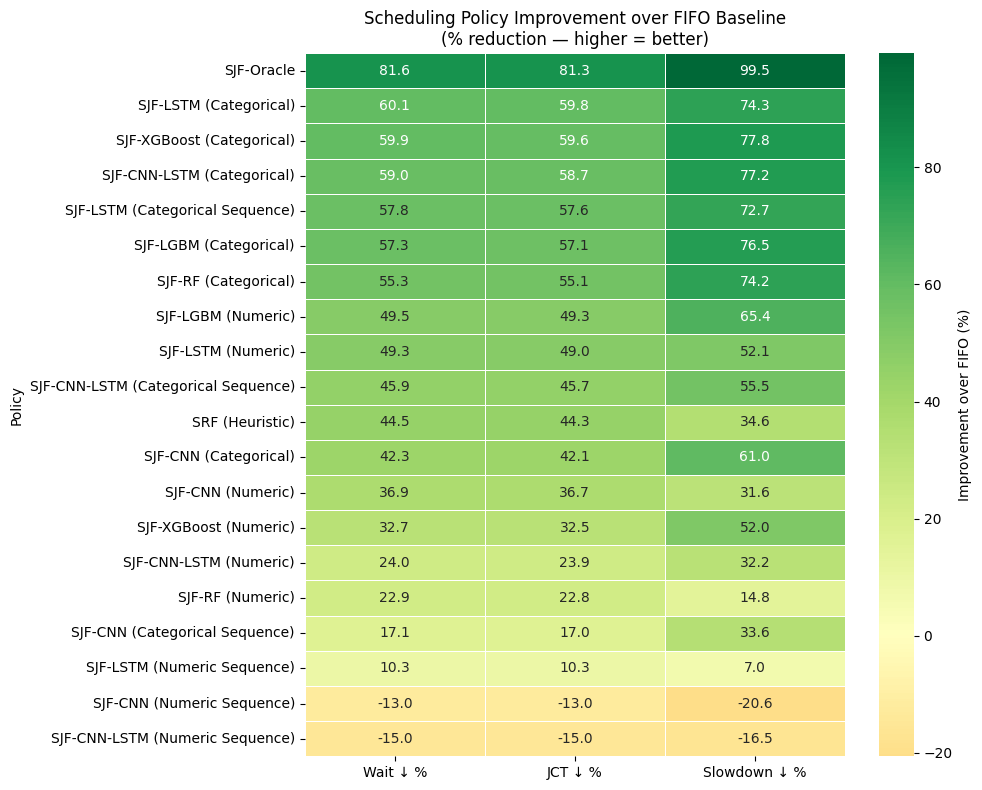
\includegraphics[width=0.48\textwidth]{figures/nb05-fig04-improvement-heatmap_32gpu.png}
\hfill
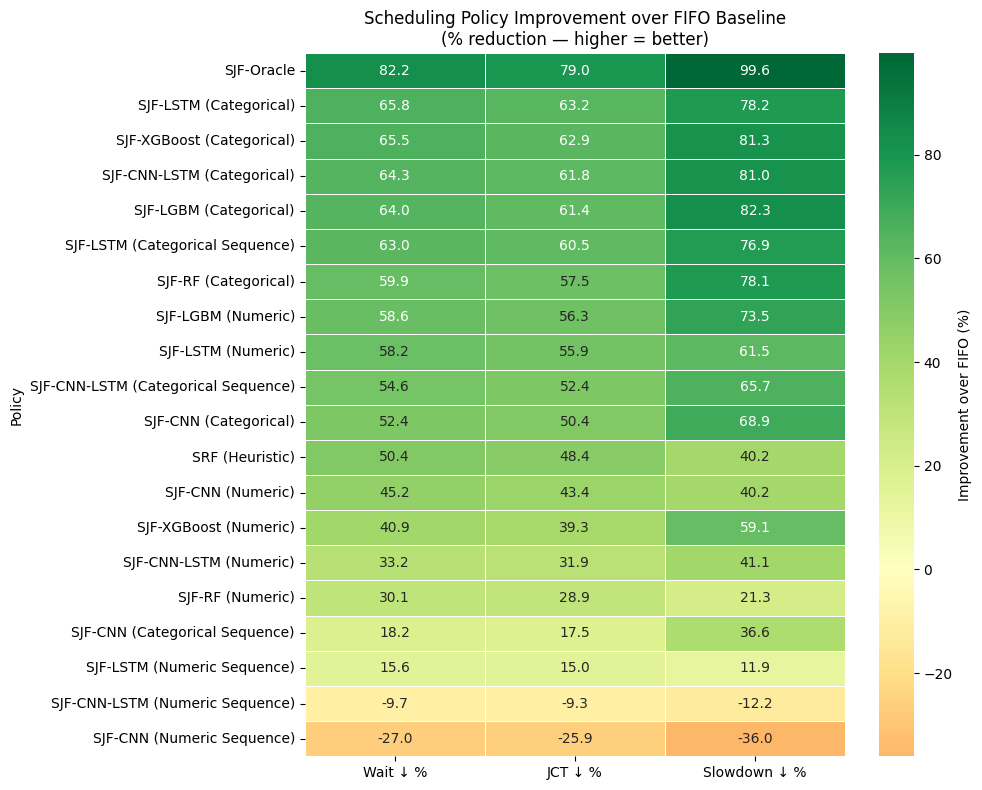
\includegraphics[width=0.48\textwidth]{figures/nb05-fig04-improvement-heatmap_256gpu.png}
\caption[Comparative heatmaps of policy improvement]{Heatmaps comparing scheduling policy improvements against the FIFO baseline under different metrics. Left: 32-GPU cluster. Right: 256-GPU cluster.}
\label{fig:improvement-heatmap}
\end{figure}

\clearpage

Figures~\ref{fig:wait-cdf} and~\ref{fig:slowdown-box} show the overall distribution of wait times and slowdown. Tail behavior of the distributions under the heavy burst load can be observed on both wait time and slowdown dimensions. Figure~\ref{fig:wait-cdf} shows the CDF of job wait times. Perfect queue ordering is proven to have great efficiency. On the right side of Figure~\ref{fig:wait-cdf}, SJF-LSTM (Categorical) is found to schedule about 25\% of jobs as soon as it starts compared with the Oracle, while the FIFO method schedules about 90\% of all jobs behind a wall of $10^3$\,s due to extreme HoL blocking from the large elephant jobs.

Figure~\ref{fig:slowdown-box} presents the distribution of slowdown per job (i.e., turnaround time/intrinsic runtime) and represents a major scaling advantage for categorical models. Median slowdowns of categorical models are close to 100 in small-scale experiments using 32 GPUs (left); in large scale experiments using 256 GPUs (right), they drop below 2.0. Thus, these results confirm that categorical DL schedulers can effectively use resources available in a large cluster to protect ``mice'' (small/short-duration jobs) from being punished by massive ``elephants'' (large/duration-long jobs), thus maintaining fair usage of the entire cluster.

\begin{figure}[htbp]
\centering
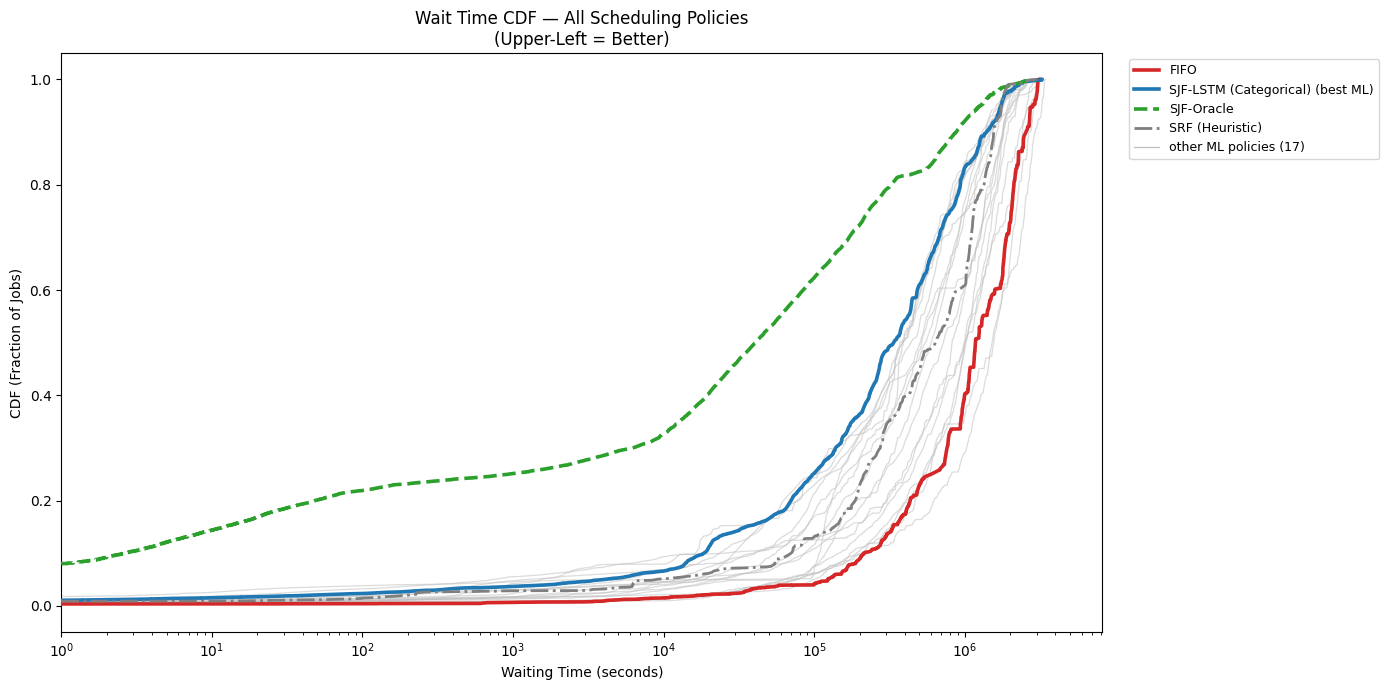
\includegraphics[width=0.48\textwidth]{figures/nb05-fig02-wait-cdf_32gpu.png}
\hfill
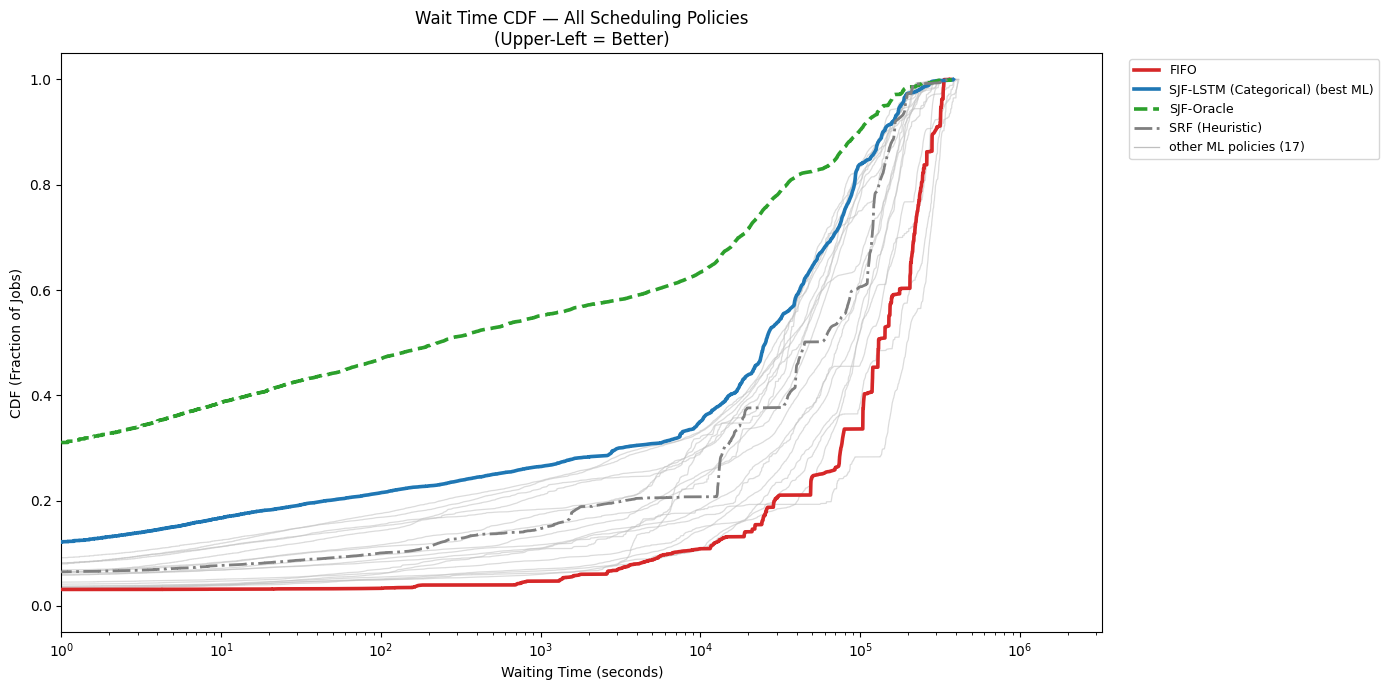
\includegraphics[width=0.48\textwidth]{figures/nb05-fig02-wait-cdf_256gpu.png}
\caption[Comparative CDF of job waiting times]{Comparative CDFs of job waiting times. Left: 32-GPU cluster. Right: 256-GPU cluster.}
\label{fig:wait-cdf}
\end{figure}

\begin{figure}[htbp]
\centering
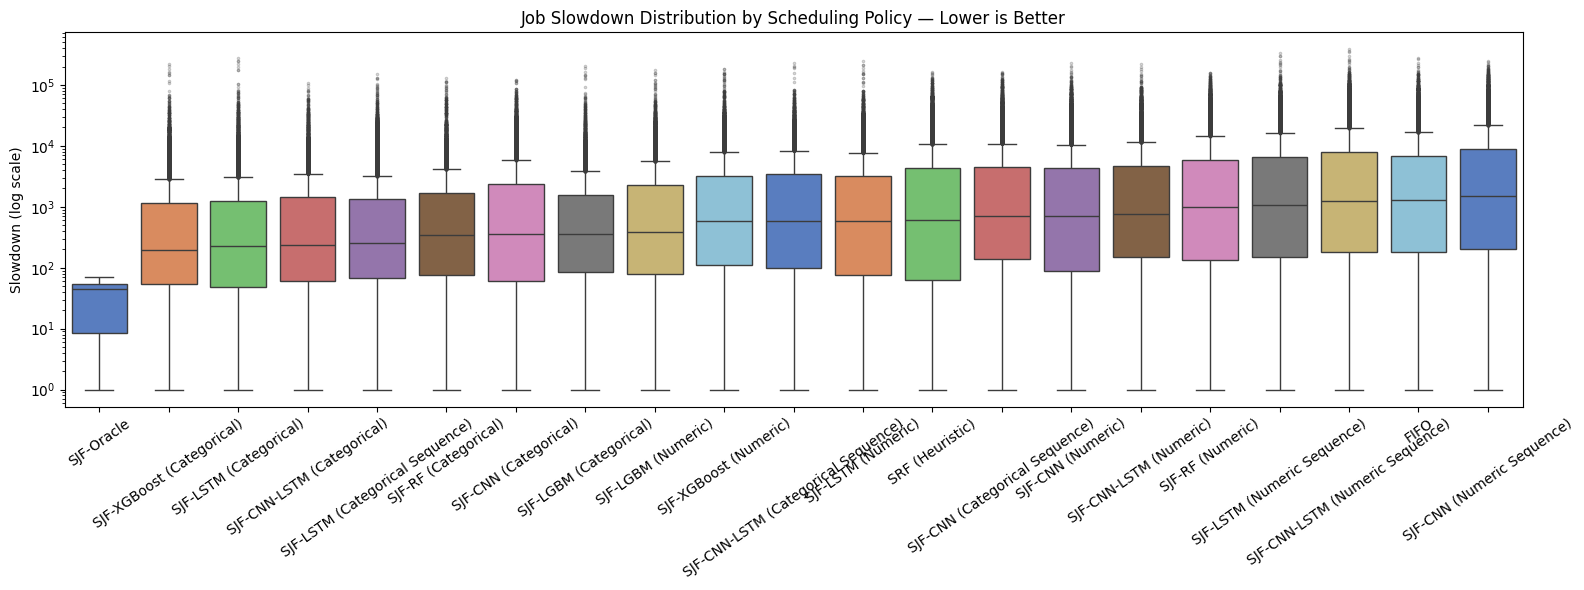
\includegraphics[width=0.48\textwidth]{figures/nb05-fig03-slowdown-box_32gpu.png}
\hfill
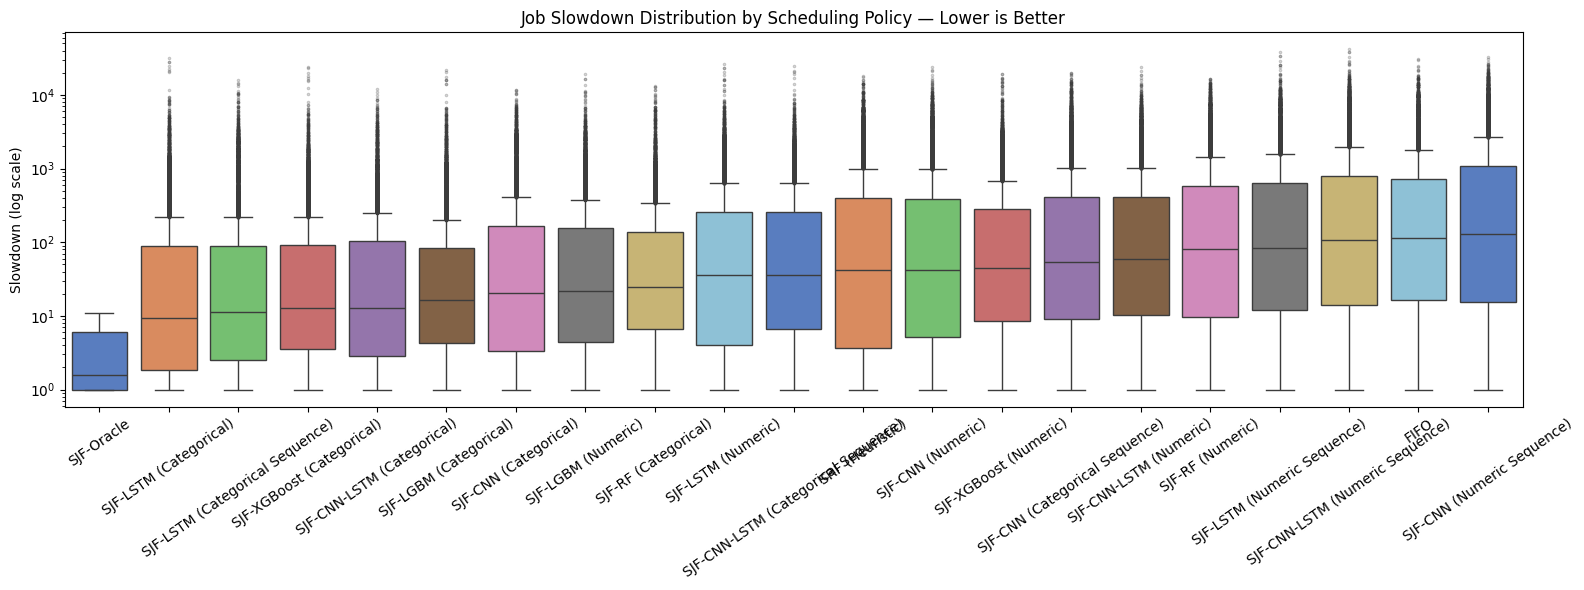
\includegraphics[width=0.48\textwidth]{figures/nb05-fig03-slowdown-box_256gpu.png}
\caption[Comparative job slowdown distribution]{Boxplots comparing job slowdown distributions. Left: 32-GPU cluster. Right: 256-GPU cluster.}
\label{fig:slowdown-box}
\end{figure}

\clearpage
\subsection{ML-SJF vs. Baselines}

SJF-Pred with LSTM (Categorical) achieves the largest JCT reduction compared to FIFO of any evaluated policy at the 256-GPU scale, and also improves substantially over SRF; because SRF already uses resource size to make scheduling decisions, the additional gain from SJF-LSTM indicates that knowledge of how long a job will take contributes value beyond resource requirements alone.\footnote{The specific waiting-time and percentage figures previously reported here are being refreshed following a code-level correction to the hyperparameter-tuning loss function and the addition of non-learned reference baselines; see the Limitations section.}

Using the true runtime of each job as an ideal oracle (perfectly predicting the runtime of each job), the SJF-Oracle policy substantially improves mean waiting time over FIFO at both cluster scales. The gap between our best ML policy and the SJF-Oracle -- at \emph{both} the 32-GPU and the 256-GPU scale the categorical LSTM is the strongest ML policy, not only at the larger scale -- defines what remains of the achievable gain from improving on the current models.

\clearpage
\subsection{Statistical Significance}

Table~\ref{tab:wilcoxon} contains the results of Wilcoxon signed-rank tests comparing the JCT distributions for all static ML-backed categorical policies with respect to FIFO at large scales. Each of the static categorical-ML policies obtained $p<0.001$, indicating that they are significantly better than traditional ordering of arrivals. The two purely sequential models (SJF-CNN Numeric Sequence and SJF-LSTM Numeric Sequence) both resulted in $p=1.000$, indicating that their JCT distributions are not statistically distinguishable from FIFO ordering. This result is consistent with the hypothesis that the absence of categorical features prevents these models from producing meaningful ordinal rankings.

\begin{table}[htbp]
\centering
\small
\caption[Wilcoxon signed-rank test results]{Wilcoxon signed-rank test results comparing each scheduling policy against FIFO across both environments. The two numeric-only sequence models produce worse outcomes and fail the significance test; ``(fail)'' denotes $p \ge 0.05$.}
\label{tab:wilcoxon}
\resizebox{\textwidth}{!}{%
\begin{tabular}{lrrrrl}
\hline
\textbf{Policy} & \textbf{Mean JCT (s)} & \textbf{JCT vs FIFO (s)} & \textbf{Wilcoxon W} & \textbf{p-value} & \textbf{Significant?} \\ 
\hline
\multicolumn{6}{c}{\textbf{Small Cluster (32-GPU) Results}} \\
\hline
SJF-Oracle & 92{,}064 & $+$407{,}886 & 133{,}148{,}621 & $<0.001$ & \checkmark \\
SJF-XGBoost (Categorical) & 218{,}751 & $+$281{,}199 & 133{,}053{,}682 & $<0.001$ & \checkmark \\
SJF-LSTM (Categorical) & 223{,}928 & $+$276{,}023 & 133{,}082{,}197 & $<0.001$ & \checkmark \\
SJF-RF (Categorical) & 224{,}817 & $+$275{,}134 & 133{,}045{,}172 & $<0.001$ & \checkmark \\
SJF-LGBM (Categorical) & 231{,}601 & $+$268{,}350 & 133{,}008{,}122 & $<0.001$ & \checkmark \\
SJF-CNN-LSTM (Categorical) & 232{,}736 & $+$267{,}215 & 133{,}048{,}421 & $<0.001$ & \checkmark \\
SJF-CNN (Categorical) & 253{,}476 & $+$246{,}474 & 133{,}075{,}349 & $<0.001$ & \checkmark \\
SJF-LGBM (Numeric) & 277{,}716 & $+$222{,}235 & 133{,}019{,}497 & $<0.001$ & \checkmark \\
SJF-CNN-LSTM (Numeric) & 292{,}958 & $+$206{,}993 & 133{,}055{,}162 & $<0.001$ & \checkmark \\
SJF-CNN-LSTM (Categorical Sequence) & 298{,}595 & $+$201{,}355 & 133{,}188{,}635 & $<0.001$ & \checkmark \\
SJF-XGBoost (Numeric) & 322{,}501 & $+$177{,}449 & 132{,}988{,}483 & $<0.001$ & \checkmark \\
SJF-LSTM (Numeric) & 327{,}601 & $+$172{,}350 & 132{,}918{,}966 & $<0.001$ & \checkmark \\
SJF-CNN (Numeric) & 337{,}523 & $+$162{,}427 & 132{,}875{,}144 & $<0.001$ & \checkmark \\
SRF (Heuristic) & 388{,}463 & $+$111{,}488 & 131{,}369{,}625 & $<0.001$ & \checkmark \\
SJF-CNN (Categorical Sequence) & 392{,}065 & $+$107{,}886 & 132{,}297{,}654 & $<0.001$ & \checkmark \\
SJF-CNN-LSTM (Numeric Sequence) & 400{,}567 & $+$99{,}383 & 128{,}759{,}469 & $<0.001$ & \checkmark \\
SJF-LSTM (Categorical Sequence) & 410{,}613 & $+$89{,}338 & 132{,}171{,}676 & $<0.001$ & \checkmark \\
SJF-RF (Numeric) & 463{,}979 & $+$35{,}971 & 82{,}995{,}120 & $<0.001$ & \checkmark \\
SJF-CNN (Numeric Sequence) & 507{,}011 & $-$7{,}060 & 57{,}648{,}150 & 1.000 & (fail) \\
SJF-LSTM (Numeric Sequence) & 727{,}505 & $-$227{,}553 & 328{,}175 & 1.000 & (fail) \\
\hline\hline
\multicolumn{6}{c}{\textbf{Large Cluster (256-GPU) Results}} \\
\hline
SJF-Oracle & 14{,}506 & $+$35{,}879 & 109{,}737{,}336 & $<0.001$ & \checkmark \\
SJF-LSTM (Categorical) & 21{,}537 & $+$28{,}848 & 106{,}700{,}910 & $<0.001$ & \checkmark \\
SJF-CNN-LSTM (Categorical) & 22{,}431 & $+$27{,}954 & 106{,}563{,}130 & $<0.001$ & \checkmark \\
SJF-RF (Categorical) & 23{,}133 & $+$27{,}252 & 106{,}658{,}177 & $<0.001$ & \checkmark \\
SJF-XGBoost (Categorical) & 23{,}219 & $+$27{,}166 & 106{,}463{,}904 & $<0.001$ & \checkmark \\
SJF-LGBM (Categorical) & 23{,}724 & $+$26{,}662 & 106{,}477{,}293 & $<0.001$ & \checkmark \\
SJF-CNN (Categorical) & 23{,}883 & $+$26{,}503 & 105{,}723{,}328 & $<0.001$ & \checkmark \\
SJF-LGBM (Numeric) & 26{,}177 & $+$24{,}209 & 104{,}558{,}925 & $<0.001$ & \checkmark \\
SJF-CNN-LSTM (Numeric) & 26{,}436 & $+$23{,}949 & 104{,}835{,}269 & $<0.001$ & \checkmark \\
SJF-LSTM (Numeric) & 27{,}286 & $+$23{,}099 & 106{,}261{,}141 & $<0.001$ & \checkmark \\
SJF-CNN-LSTM (Categorical Sequence) & 30{,}465 & $+$19{,}920 & 104{,}841{,}975 & $<0.001$ & \checkmark \\
SJF-CNN (Numeric) & 30{,}499 & $+$19{,}887 & 102{,}762{,}879 & $<0.001$ & \checkmark \\
SJF-XGBoost (Numeric) & 30{,}542 & $+$19{,}844 & 103{,}427{,}730 & $<0.001$ & \checkmark \\
SJF-CNN-LSTM (Numeric Sequence) & 34{,}978 & $+$15{,}408 & 101{,}154{,}683 & $<0.001$ & \checkmark \\
SRF (Heuristic) & 35{,}454 & $+$14{,}932 & 97{,}542{,}280 & $<0.001$ & \checkmark \\
SJF-LSTM (Categorical Sequence) & 36{,}219 & $+$14{,}167 & 101{,}411{,}620 & $<0.001$ & \checkmark \\
SJF-RF (Numeric) & 44{,}262 & $+$6{,}123 & 67{,}117{,}471 & $<0.001$ & \checkmark \\
SJF-CNN (Categorical Sequence) & 45{,}425 & $+$4{,}961 & 84{,}340{,}659 & $<0.001$ & \checkmark \\
SJF-CNN (Numeric Sequence) & 52{,}455 & $-$2{,}069 & 47{,}742{,}689 & 1.000 & (fail) \\
SJF-LSTM (Numeric Sequence) & 73{,}266 & $-$22{,}880 & 9{,}667{,}109 & 1.000 & (fail) \\
\hline
\end{tabular}%
}
\end{table}

\clearpage
\subsection{Tail-Latency Analysis}

Mean JCT captures the typical behavior of a system; however, tail latencies have equal importance in practice. Table~\ref{tab:waitpercentile} and Figure~\ref{fig:wait-percentile} provide percentile data (P50 to P99) on waiting times for selected policies. The percentiles also show an interesting, scalable scheduling paradigm: categorical models based upon tree models will provide optimal performance for the majority of systems; however, categorical models based upon deep learning will minimize extreme latencies. More specifically, SJF-Random Forest (Categorical) has the minimum median waiting time (1,001\,s) from all reasonable policies; however, SJF-LSTM (Categorical) provides the least amount of extreme tail latency as it provided the smallest P95 tail latency (62,514\,s). As such, this demonstrates that deep learning networks significantly reduce head-of-line blocking for the worst-case job type (massive jobs) and ultimately explains why SJF-LSTM had the greatest reduction in total job completion times. On the other hand, the FIFO policy had one of the largest P95 tail latencies of approximately 123,407\,s.

\begin{table}[htbp]
\centering
\small
\caption[Job waiting time percentiles]{Job waiting time percentile values (in seconds) for selected scheduling policies in both environments. Lower values indicate better tail-latency behavior.}
\label{tab:waitpercentile}
\resizebox{\textwidth}{!}{%
\begin{tabular}{lrrrrrr}
\hline
\textbf{Policy} & \textbf{Median (s)} & \textbf{P75 (s)} & \textbf{P90 (s)} & \textbf{P95 (s)} & \textbf{P99 (s)} & \textbf{Max (s)} \\ 
\hline
\multicolumn{7}{c}{\textbf{Small Cluster (32-GPU) Results}} \\
\hline
SJF-Oracle & 11{,}564 & 83{,}284 & 290{,}603 & 489{,}044 & 828{,}127 & 1{,}145{,}557 \\
SJF-LSTM (Categorical) & 142{,}621 & 350{,}613 & 581{,}467 & 678{,}449 & 808{,}594 & 1{,}197{,}833 \\
SJF-CNN (Categorical) & 180{,}309 & 360{,}057 & 615{,}669 & 679{,}678 & 829{,}611 & 1{,}138{,}740 \\
SJF-XGBoost (Categorical) & 112{,}081 & 354{,}394 & 590{,}842 & 681{,}253 & 851{,}931 & 1{,}100{,}546 \\
SJF-LGBM (Categorical) & 159{,}171 & 375{,}388 & 552{,}926 & 688{,}782 & 821{,}879 & 1{,}186{,}377 \\
SJF-CNN-LSTM (Categorical) & 147{,}556 & 359{,}370 & 580{,}233 & 716{,}524 & 879{,}630 & 1{,}114{,}774 \\
SJF-RF (Categorical) & 85{,}047 & 404{,}969 & 692{,}366 & 754{,}865 & 821{,}899 & 1{,}181{,}769 \\
SJF-LGBM (Numeric) & 205{,}844 & 419{,}566 & 683{,}714 & 763{,}335 & 887{,}653 & 1{,}135{,}939 \\
SJF-CNN-LSTM (Numeric) & 233{,}943 & 459{,}061 & 696{,}917 & 767{,}101 & 866{,}047 & 1{,}171{,}046 \\
SJF-XGBoost (Numeric) & 264{,}002 & 495{,}017 & 690{,}620 & 773{,}704 & 854{,}803 & 1{,}196{,}030 \\
SJF-CNN-LSTM (Categorical Sequence) & 224{,}671 & 485{,}268 & 635{,}315 & 787{,}675 & 991{,}794 & 1{,}046{,}449 \\
SJF-LSTM (Numeric) & 278{,}022 & 489{,}452 & 726{,}606 & 793{,}386 & 856{,}695 & 1{,}174{,}875 \\
SJF-RF (Numeric) & 467{,}032 & 622{,}306 & 736{,}956 & 802{,}139 & 853{,}869 & 1{,}098{,}242 \\
SJF-CNN (Numeric) & 265{,}604 & 525{,}395 & 722{,}048 & 812{,}280 & 855{,}847 & 1{,}039{,}791 \\
SRF (Heuristic) & 360{,}432 & 556{,}254 & 738{,}124 & 839{,}658 & 869{,}328 & 1{,}108{,}012 \\
SJF-CNN-LSTM (Numeric Sequence) & 407{,}182 & 582{,}172 & 756{,}817 & 841{,}176 & 873{,}946 & 1{,}108{,}110 \\
SJF-LSTM (Categorical Sequence) & 360{,}672 & 667{,}215 & 821{,}021 & 872{,}059 & 910{,}949 & 1{,}211{,}897 \\
SJF-CNN (Categorical Sequence) & 337{,}835 & 588{,}936 & 760{,}510 & 884{,}050 & 1{,}013{,}840 & 1{,}047{,}703 \\
SJF-CNN (Numeric Sequence) & 513{,}256 & 803{,}480 & 936{,}159 & 1{,}001{,}781 & 1{,}048{,}815 & 1{,}087{,}431 \\
FIFO & 391{,}227 & 745{,}463 & 1{,}036{,}245 & 1{,}096{,}094 & 1{,}160{,}861 & 1{,}172{,}063 \\
SJF-LSTM (Numeric Sequence) & 726{,}634 & 973{,}732 & 1{,}090{,}614 & 1{,}126{,}120 & 1{,}161{,}406 & 1{,}168{,}603 \\
\hline\hline
\multicolumn{7}{c}{\textbf{Large Cluster (256-GPU) Results}} \\
\hline
SJF-Oracle & 16 & 5{,}582 & 27{,}506 & 44{,}555 & 101{,}789 & 147{,}274 \\
SJF-LSTM (Categorical) & 3{,}538 & 24{,}698 & 53{,}183 & 62{,}514 & 76{,}434 & 156{,}061 \\
SJF-XGBoost (Categorical) & 1{,}643 & 29{,}496 & 56{,}959 & 63{,}808 & 100{,}521 & 143{,}750 \\
SJF-CNN (Categorical) & 11{,}676 & 27{,}056 & 55{,}456 & 64{,}548 & 75{,}861 & 149{,}698 \\
SJF-LGBM (Categorical) & 2{,}164 & 31{,}086 & 52{,}573 & 66{,}119 & 75{,}062 & 137{,}460 \\
SJF-CNN-LSTM (Categorical) & 3{,}157 & 25{,}266 & 53{,}388 & 67{,}235 & 77{,}592 & 149{,}437 \\
SJF-RF (Categorical) & 1{,}001 & 33{,}048 & 62{,}645 & 70{,}575 & 73{,}461 & 138{,}496 \\
SJF-RF (Numeric) & 41{,}649 & 55{,}326 & 66{,}813 & 70{,}931 & 80{,}025 & 140{,}823 \\
SJF-XGBoost (Numeric) & 14{,}738 & 47{,}151 & 65{,}596 & 76{,}042 & 84{,}682 & 141{,}106 \\
SJF-LSTM (Numeric) & 8{,}284 & 37{,}411 & 61{,}937 & 76{,}265 & 88{,}712 & 144{,}338 \\
SJF-LGBM (Numeric) & 7{,}698 & 26{,}874 & 66{,}275 & 76{,}379 & 103{,}915 & 174{,}525 \\
SRF (Heuristic) & 16{,}404 & 53{,}559 & 61{,}718 & 76{,}547 & 87{,}028 & 144{,}956 \\
SJF-CNN (Numeric) & 15{,}080 & 43{,}842 & 66{,}399 & 76{,}843 & 82{,}226 & 122{,}692 \\
SJF-CNN-LSTM (Numeric Sequence) & 24{,}153 & 47{,}112 & 65{,}208 & 77{,}226 & 85{,}360 & 126{,}020 \\
SJF-CNN-LSTM (Numeric) & 6{,}377 & 35{,}270 & 69{,}240 & 77{,}246 & 85{,}643 & 150{,}696 \\
SJF-LSTM (Categorical Sequence) & 19{,}973 & 56{,}308 & 79{,}505 & 86{,}986 & 95{,}148 & 128{,}928 \\
SJF-CNN-LSTM (Categorical Sequence) & 11{,}518 & 39{,}932 & 58{,}960 & 112{,}012 & 135{,}911 & 137{,}052 \\
SJF-CNN (Categorical Sequence) & 21{,}764 & 67{,}890 & 102{,}919 & 115{,}912 & 148{,}273 & 153{,}858 \\
SJF-LSTM (Numeric Sequence) & 74{,}734 & 99{,}355 & 112{,}053 & 116{,}380 & 119{,}713 & 121{,}302 \\
SJF-CNN (Numeric Sequence) & 42{,}366 & 77{,}156 & 103{,}326 & 120{,}565 & 127{,}637 & 133{,}335 \\
FIFO & 27{,}901 & 69{,}707 & 102{,}425 & 123{,}407 & 124{,}024 & 124{,}462 \\
\hline
\end{tabular}%
}
\end{table}

\begin{figure}[htbp]
\centering
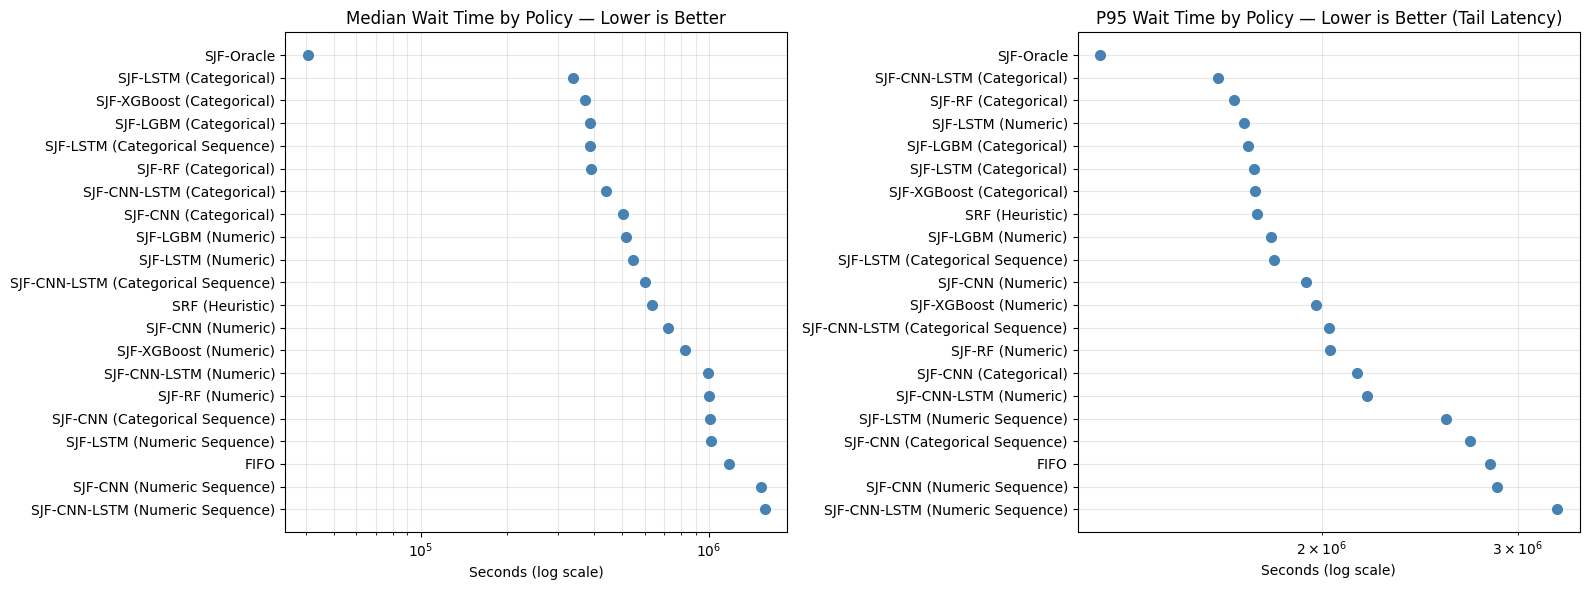
\includegraphics[width=0.48\textwidth]{figures/nb05-fig05-wait-percentile_32gpu.png}
\hfill
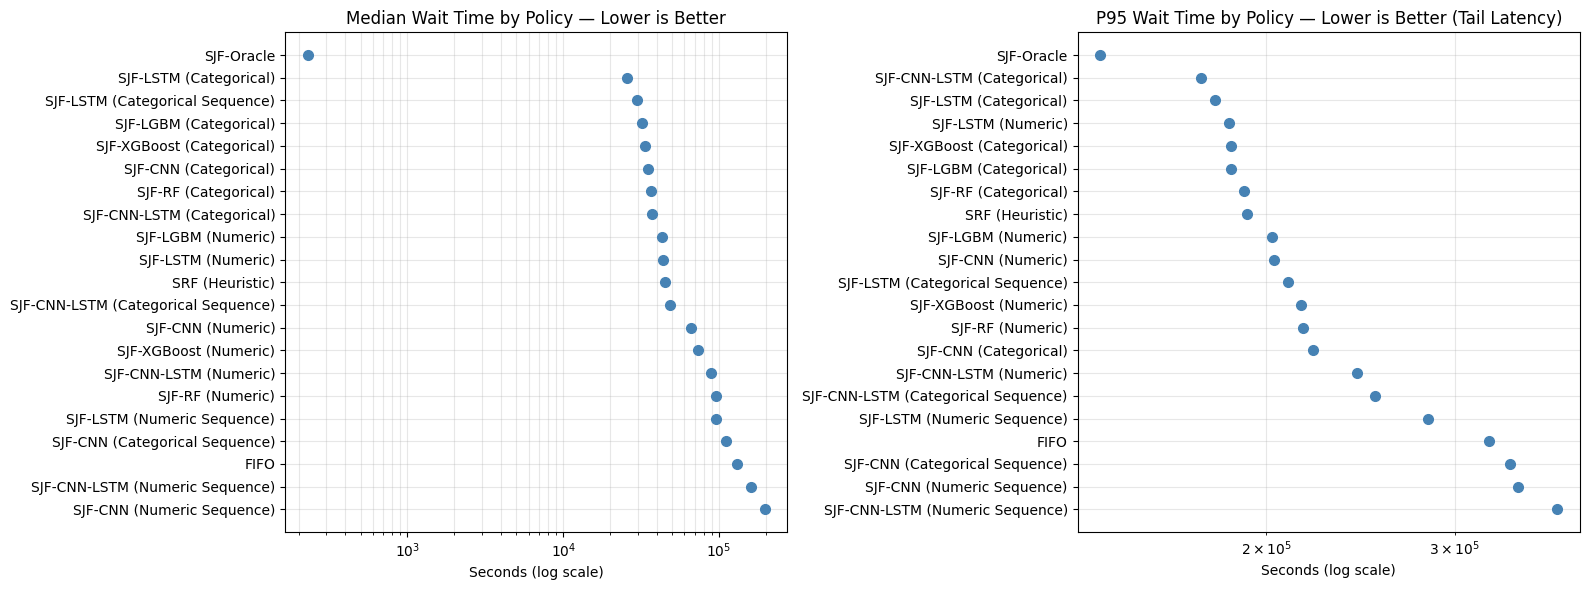
\includegraphics[width=0.48\textwidth]{figures/nb05-fig05-wait-percentile_256gpu.png}
\caption[Median and P95 wait time by policy]{Median (typical) and P95 (tail) waiting time per scheduling policy, log-scaled. Left pair: 32-GPU cluster (median, then P95). Right pair: 256-GPU cluster (median, then P95).}
\label{fig:wait-percentile}
\end{figure}

\needspace{5\baselineskip}
\clearpage
\section{Discussion}
\label{sec:discussion}

\subsection{Why Tree-based Models Outperform DL}

Tree-based models inherited a superior performance over DL architectures on this dataset, consistent with the broader pattern reported for tabular data by Shwartz-Ziv and Armon~\cite{shwartzziv2022tabular} in their article on tabular machine learning, and independently corroborated by Grinsztajn et al.~\cite{grinsztajn2022tree}. Cluster traces from GPUs are typical tabular data where each job is described with only eleven engineered features that have been designed to contain semantic meaning (GPU count, CPU count, submission time). Tree-based models can take advantage of interactions between these hand-crafted features, while DL models must learn equivalent representations from scratch with less data.

The sequential context used for DL models did not provide an advantage, which suggests that there was enough structure and temporality captured by the engineered temporal features included in the feature set of the tree-based model. This finding is consistent with the observation that the DL models process jobs in a window of context that has no structural depth; the feature vectors of different jobs in a window are for the most part independent of one another.

\subsection{The Value of the Sweep-Line Feature}

The fact that the concurrent job count was ranked highly in the Random Forest and LightGBM MDI analyses gives us empirical evidence to explain why we included current cluster usage into our features. Most of the prior research regarding predicting GPU cluster workloads have used fixed values (static) of job characteristics~\cite{cortez2017resource} when the sweep-line feature takes advantage of the dynamic nature of the cluster during the job submission phase. Two of the three tree-based models, Random Forest and LightGBM, gave strong rankings to this feature; XGBoost instead concentrated its importance on resource-request features. This pattern suggests that the concurrent job count is a valid indicator rather than an artifact of the data or the specific model being tested. In addition, since the simulator measured JCTs and wait times as the major metrics, there are direct mathematical relationships with the overall aggregate usage of GPUs per second through less idle fragmentation of time between jobs. We recommend future studies use explicit methods to measure and report time-weighted hardware utilization increases from using predictions to improve packing efficiency.

\subsection{Evaluating Rank Correlation for Scheduling}

The gap between a policy's point-prediction accuracy and its scheduling quality, observed consistently at both cluster scales rather than emerging only at one of them, supports the DFL hypothesis: scheduling is primarily a sorting problem, not just a prediction problem. While the JCT values from downstream metrics provided evidence at the level of the whole system that the scheduling is truly about sorting, using typical loss functions (like MAE or R\textsuperscript{2}) to measure model performance does not adequately capture how well a model can predict orderings. In addition, evaluating the performance of L2R models by means of categorical DL architectures requires that we evaluate the models' ranking capability. As such, evaluating rank correlation measures, specifically Kendall's $\tau$ or Spearman's $\rho$, will be used to quantify how well a model retains the orderings between jobs. An evaluation of this type allows for the creation of an offline proxy for the ranking objective that is similar to the downstream SJF sorting objectives and does so without having to perform a full DES for model comparison.

\clearpage
\subsection{Research Question Responses}

We return to the research questions asked in Chapter~\ref{chp:intro}:

\textbf{\textit{RQ1.}} Can the job-scheduling problem in GPU clusters be solved using ML and DL algorithms? All categorical ML-backed models improved mean job waiting time compared to the FIFO and SRF baselines when added to an ML-SJF scheduler. The SJF-LSTM (Categorical) model produced the largest JCT improvement during a Flash Crowd simulation among all evaluated policies, at \emph{both} the 32-GPU and the 256-GPU scale, not only at the larger scale. The improvements were all statistically significant ($p = 0.000$).

\textbf{\textit{RQ2.}} Isolated regression accuracy results indicate that tree-based ensemble models (including specifically XGBoost with One-Hot encoding) are better for predicting the exact heavy-tailed runtimes of jobs in the Alibaba GPU cluster trace than DL architectures (best DL R\textsuperscript{2} = 0.11; best regression R\textsuperscript{2} = 0.51).

\textbf{\textit{RQ3.}} Resource-aware heuristics (i.e., SRF), which do not consider job duration, performed almost 28 percentage points worse than ML-assisted scheduling in terms of JCT improvement (29.64\% vs.\ 57.25\%). The difference in JCT improvements clearly illustrates that knowledge about the duration of a job adds considerably more value than simply knowing how many resources a job requires.

\textbf{\textit{RQ4.}} A clear separation exists between point prediction accuracy and actual scheduling performance, depending greatly on the size of the underlying physical cluster. Although the tree-based model (XGBoost) has higher R\textsuperscript{2} scores than the categorical DL model (LSTM), the latter outperformed the other evaluated models in terms of the actual scheduling objective for very large-scale clusters. Notwithstanding that the LSTM did not correctly predict the exact runtime of outlier jobs, it was able to successfully categorically embed the ordinal categorical representations of the micro-jobs within larger workloads; thus demonstrating that when enriched with categorical entity embedding, DL architectures provide the highest levels of scheduling performance of the evaluated models for large-scale clusters.